\documentclass[11pt]{article}
% NSF PAPPG Ch. 2 §B.2: font ≥11pt, margins ≥1in, ≤6 lines/inch.
% No hyperlinks in Project Description body (Research.gov constraint).
% Proposal title (Research.gov submission form, not part of this file's typeset content):
% CPS-CIR: Closing the Cyber-Physical Loop between Community Knowledge and
% Hydrological Modeling for Flood-Resilient Historic Communities

\usepackage{amsmath}
\usepackage{bm}
\usepackage{color}
\usepackage{hyperref}
\usepackage{graphicx}
\usepackage{wrapfig}
\usepackage{subcaption}
\usepackage{vmargin}
\usepackage{mathrsfs}
\usepackage{float}
\usepackage{tabularx}
\usepackage{booktabs} 
\usepackage{longtable}
\usepackage{ltablex}
\usepackage[svgnames]{xcolor}
\usepackage[most]{tcolorbox}
\usepackage{enumitem}
\usepackage{titlesec}
\usepackage{caption}
\usepackage{colortbl}
\usepackage{soul}
\sethlcolor{yellow}
\usepackage{pgfgantt}
\usepackage[numbers,square,sort&compress]{natbib}
\linespread{0.901}

% ── Colors ───────────────────────────────────────────────────────────────────
\definecolor{mycmykcolor}{cmyk}{0.45,0.30,0.20,0}
\definecolor{secondary}{cmyk}{0,0,0,0.20}
\definecolor{roonecol}{HTML}{8C9EB2}
\definecolor{rootwocol}{HTML}{E0914D}

% ── Section formatting ────────────────────────────────────────────────────────
\titleformat{\section}[runin]{\normalfont\bfseries}{\thesection}{1em}{}[:]
\titlespacing*{\section}{0pt}{\baselineskip}{1ex}
\titleformat{\subsection}[runin]{\normalfont\bfseries}{\thesubsection}{1em}{}[:]
\titlespacing*{\subsection}{0pt}{\baselineskip}{1ex}

% ── Page layout ───────────────────────────────────────────────────────────────
\bibliographystyle{unsrtnat}
\hypersetup{hidelinks,colorlinks=false,urlcolor=black}
\hypersetup{draft}
\setpapersize{USletter}
\setmarginsrb{1in}{1in}{1in}{1in}{0pt}{0mm}{0pt}{0mm}
\pretolerance=5000
\tolerance=9000
\graphicspath{{images/}}

\newcommand{\placeholder}[1]{\textcolor{red}{[\textbf{PLACEHOLDER:} #1]}}
\newcommand{\pseudodot}{{\lower 2.4pt\hbox{$\cdot$}}}

\begin{document}
% \pagestyle{empty} % turn back on for nsf
\setlength{\baselineskip}{12.6pt}
\setlength{\normalbaselineskip}{12.6pt}

% ============================================================
%  PROJECT GOALS BOX
% ============================================================

\begin{tcolorbox}[colback=mycmykcolor, colframe=black, boxrule=1pt, coltext=black]
\textbf{Project goals:}
Small, repeatedly-flooded municipalities with older building stock have no
engineering tool to evaluate whether community-scale drainage investment or distributed
building hardening better reduces flood damage.
Here we propose a closed-loop cyber-physical system (CPS) that couples the physical
behavior of pre-code load-bearing masonry and timber, absent from existing fragility
frameworks, with a computational core that turns free national data and community
memory into building-level damage estimates. It senses through USGS gauges and NOAA
precipitation operationally, with commercial ICEYE Synthetic Aperture Radar (SAR) for
one-time building-level duration and depth calibration and open Sentinel-1 SAR for
flood-extent context; its computational core is a Bayesian uncertainty-quantification
framework fusing a GIS-parameterizable mass balance model, one whose inputs come
entirely from free national GIS data layers (USGS 3DEP, NLCD, SSURGO, NHD
StreamStats) rather than locally calibrated hydraulic models, with community-elicited
duration priors and a gauge-stage-to-terrain projection for building-level depth; and
the community closes the loop through a co-developed two-mode interface for scenario-based retrofit planning, forecast-driven staging, and post-event model updating.
\textbf{RQ1} (Napolitano, Wauthier, and Busse) asks to what extent this CPS,
operating on free national data and community knowledge, can produce building-level
damage assessments decision-adequate to weigh community-scale drainage against
building-scale hardening on a common probabilistic basis, without hydraulic
simulation.
\textbf{RQ2} (Napolitano with input from all PIs) asks under what conditions locally held
community knowledge, entered as Bayesian calibration priors, improves damage
assessments relative to a GIS-only baseline, and where it functions as a substitute
versus complement to geospatial data.
The intellectual contribution is the closed loop these questions form, in which free
national data and community knowledge together support real investment decisions, with
community knowledge a structural calibration input measured against a geospatial
baseline, the Community-Inspired Research (CIR) component of this CPS.
\end{tcolorbox}
\vspace{-0.5cm}
\normalsize

% ============================================================
%  STATUS QUO
% ============================================================

\section{Status quo}
Small communities at the confluence of riverine flood hazard and older building
stock face a resilience challenge that no existing engineering framework is designed
to address.
Across the northeastern United States and Appalachian corridor, thousands of towns
share this profile of multi-day riverine flood exposure, older load-bearing masonry
and timber cores, and institutional capacity below the threshold for hydrodynamic
simulation \cite{smith2013statecapacity,horney2012ruralstatus}.
Of the more than 22,000 communities FEMA's National Flood Insurance Program enrolls
nationwide \cite{horn2024nfip}, thousands in this region combine significant
pre-1940 building stock, no in-house hydraulic modeling capacity, and repeated
riverine flooding.
In Vermont alone, over a quarter of the housing stock predates 1939
\cite{census2017b25034,vhfa2020housingneeds}.
For these communities, every flood event surfaces the same unresolved question.
Where do limited flood-mitigation dollars belong?

These communities face a menu of mitigation choices, most of them permanent
investments and a few made in the hours before a storm.
What they lack is any way to weigh those choices on a common probabilistic footing,
using the assets they actually have, a handful of physical sensors, some public
geospatial data, and a deep store of community memory.
The sharpest case is the allocation question.
Would a community-scale drainage investment, such as a retention basin, reduce damage
enough to justify its cost over the same dollars spent hardening individual buildings?
Answering it means linking an upstream drainage decision to downstream building
damage probabilities, a comparison no existing framework lets a small community make.

That comparison demands two things these communities do not have.
The first is a model.
Hydrodynamic simulation pipelines such as HEC-RAS and LISFLOOD-FP require calibrated
hydraulic models, high-resolution topographic data, and sustained technical staff
that small towns cannot maintain \cite{usace2024hecras,bates2000lisflood,fewtrell2011benchmarking}.
The second is data on how their own buildings fail.
Damage functions in HAZUS and FEMA P-58 are built around post-1945 construction, so
the load-bearing masonry and timber structures built before modern building codes
(pre-code), the dominant type in repeatedly flooded historic downtowns, are absent
from existing fragility frameworks \cite{fema2025hazus,fema2018p58}.
Those frameworks also treat damage as a function of depth alone, not the
extended-inundation degradation that governs older masonry, which we review in the
fragility state of the art below.
Even the most authoritative federal guidance on functional recovery, NIST SP~1310
\cite{davis2024nist}, concedes that its framework is too complex for smaller agencies
with limited resources and funding, and calls for simplifications that smaller
organizations can actually implement \cite[Sec.~6.1.3]{davis2024nist}.
Emergency managers, preservation officials, and building owners have no engineering
tool that turns a flood event into building-specific guidance.

What these towns lack in models and data, they hold in memory.
Residents know how deep the water rose, how long it stayed, which buildings took the
worst of it, and how often it returns.
Existing community resilience frameworks are largely top-down, built around
standardized data collection and modeling pipelines that resource-constrained
localities cannot sustain, and none gives a community a way to put this knowledge
into an engineering-grade probabilistic assessment.
We treat that knowledge not as context but as a calibration input, locally held flood
memory entered as Bayesian priors, whose contribution to a damage assessment can be
measured directly against a baseline built from geospatial data alone.
Building that measurement into a working loop, from free national data and community
memory to a damage estimate a town can act on, is the work that follows.

\vspace{-10pt}
\subsection{Research questions and intellectual merit}

\begin{itemize}[leftmargin=1.5em,itemsep=0pt]
\item \textbf{RQ1 (Napolitano, Wauthier, and Busse):} To what extent can a CPS
operating on free national data and community knowledge, without hydraulic
simulation, produce building-level damage assessments decision-adequate to weigh
community-scale drainage against building-scale hardening on a common probabilistic
basis?
\item \textbf{RQ2 (Napolitano with input from all PIs):} Under what conditions does locally
held community knowledge, entered as Bayesian calibration priors, improve flood
damage assessment accuracy and calibration relative to a GIS-only baseline, and
where does it function as a substitute versus complement to geospatial data?
\end{itemize}

The central contribution is the closed loop these questions form, a working
cyber-physical system in which free national data and locally held community memory
together produce building-level damage assessments decision-adequate for real
investment choices, with no hydraulic simulation anywhere in the loop. Realizing it
required three advances that did not exist for this setting. The first is
\textbf{computational}, a Bayesian framework that infers building-level inundation
depth and duration from sparse, indirect, interval-censored observations (gauge stage
projected across terrain, SAR duration brackets), fuses them with a
GIS-parameterizable mass balance model and community-elicited priors, and propagates
uncertainty to a decision-adequate damage estimate. The second is \textbf{physical}. The CPS couples to its environment on both ends, sensing physical flood signatures
(inundation depth, how long the water stayed, resulting damage) and informing physical
interventions (drainage retrofits that shorten a sub-basin's drainage timescale,
building hardening that raises the masonry capacity threshold) whose effects reenter
future flood behavior. The third is treating locally held \textbf{community knowledge}
as a structural calibration input, a characterization of when knowledge entered as
Bayesian priors improves accuracy and calibration over a GIS-only baseline, and where
it functions as a substitute versus a complement to geospatial data. Together these
establish a generalizable principle, that free national data fused with community
knowledge is sufficient for the investment decisions small municipalities face,
transferable to any domain with national data and community knowledge but no
simulation capacity.


% ============================================================
%  CURRENT STATE OF THE ART
% ============================================================

\vspace{-5pt}
\section{Current state-of-the-art}

Closing the loop requires four capabilities, estimating how long
water stays at building level, translating duration into structural
damage for the affected building stock, calibrating with community
knowledge where data are sparse, and converting damage probabilities
into investment decisions whose outcomes feed back into the next event.
Each has a mature literature, and yet none addresses the interfaces
among all four. The broader CPS literature does not close it either. Community
sensing architectures for flood monitoring assume local sensor
infrastructure, proprietary data contracts, or sustained community
effort that resource-constrained municipalities cannot maintain after
a grant ends, and none carries the community knowledge mechanism,
independent ground truth, or physical damage model the loop requires.

\subsection{Hydrological mass balance modeling and flood duration estimation}
Hydrological mass balance models estimate flood volume, storage, and drainage
timescale from watershed geometry, land cover, soil properties, and precipitation
inputs.
Unit hydrograph methods and rational method variants provide event-scale peak
discharge and runoff volume estimates for small watersheds from tabulated curve
numbers and contributing area \cite{usdascs1986tr55}; GIS-parameterized implementations using USGS
StreamStats, NHD Plus, NLCD, and SSURGO extend these approaches to ungauged
and lightly gauged basins without local calibration data
\cite{ries2017streamstats,moore2019nhdplus}.
Prior work has applied these methods to estimate peak discharge and flood extent
at community scale; their application to building-level inundation duration
estimation, the input required by duration-dependent fragility models, has not
been characterized.
Whether a GIS-only mass balance model can produce building-scale drainage timescale
estimates accurate enough for retrofit allocation where calibrated hydraulic models
are unavailable is unknown (Subtask~1.2).
% maggie: expand with key references supporting the linear-reservoir form with fractional-storage closure now committed in eq:tau (or your preferred alternative). 1-2 additional paragraphs.

\subsection{Fragility and vulnerability frameworks for flood damage}
Flood fragility and vulnerability assessment relies predominantly on depth-damage
functions that map peak inundation depth to expected repair cost or damage ratio
by occupancy class.
The HAZUS flood technical manual provides the most widely used depth-damage curves
for the United States, organized by building occupancy and foundation type
\cite{fema2025hazus};
comparable databases have been developed in Europe and Australia for loss estimation
in community-scale flood events \cite{huizinga2017jrc,gerl2016review}.
These functions share a structural assumption. Peak depth is the governing mechanical
input, and damage accumulates instantaneously at flood peak rather than over the
inundation period.
For post-1945 wood-frame and light steel construction that assumption is
approximately correct; for pre-code load-bearing masonry and timber construction
it is not.
Extended inundation drives duration-dependent degradation, including mortar
softening, progressive brick saturation, and rising damp, that depth-damage
functions cannot capture
\cite{franzoni2015compressive,sathiparan2018effect,hall2009water}.
Observational studies of masonry buildings in European riverine flood events have
documented that damage state is better predicted by depth and duration together
than by depth alone
\cite{kelman2004overview,schwarz2008damage,milanesi2018vulnerability}, yet no
duration-dependent fragility surface exists for the pre-code load-bearing masonry
archetypes that dominate repeatedly flooded northeastern American historic cores.
This absence blocks CPS integration. A duration-producing computational core needs
duration-dependent fragility, which no existing framework provides for
this building stock.
% resolved 2026-07-22: HAZUS manual, JRC/Gerl depth-damage databases, European masonry duration studies (Kelman & Spence 2004, Schwarz & Maiwald 2008, Milanesi 2018), and degradation mechanism refs (Hall & Hoff, Franzoni 2015, Sathiparan 2018) all added, verified against publisher records.

\subsection{Community knowledge in probabilistic risk assessment}
Community knowledge, local observation, and resident experience constitute a
substantial information resource for disaster risk assessment that formal modeling
pipelines largely bypass.
The Sendai Framework for Disaster Risk Reduction explicitly prioritizes
community-based approaches \cite{undrr2015sendai}; community-based disaster risk reduction programs have
demonstrated that locally held knowledge can identify hazard exposures, vulnerable
populations, and infrastructure conditions that national datasets do not capture
\cite{twigg2015disaster}.
In flood risk specifically, participatory GIS methods and volunteered geographic
information platforms have been used to map inundation extents, document damage,
and supplement remotely sensed observations \cite{goodchild2007citizens,assumpcao2018citizen}.
Existing approaches use community knowledge for post-hoc validation, qualitative
prioritization, or supplementary narrative, treating the tacit process knowledge
that residents hold about local drainage as anecdote rather than data. None
operationalizes it as a structural, quantitative calibration input to a
probabilistic building damage model.
The Bayesian prior elicitation literature provides a principled mechanism for
translating expert and stakeholder judgment into probability distributions
\cite{ohagan2006uncertain,garthwaite2005statistical}, shown elsewhere to improve
model calibration when data are sparse, but not yet applied to community flood
knowledge.
Whether community knowledge and GIS data function as substitutes, complements, or
redundant sources across building and drainage contexts remains entirely untested.
% resolved 2026-07-22 except SCC papers: Sendai, CBDRR (Twigg 2015), PGIS/VGI (Goodchild 2007, Assumpcao 2018), and elicitation (O'Hagan 2006, Garthwaite 2005) added, verified. SCC community-knowledge papers still pending, tracked with the other SCC placeholder comments.

\subsection{Flood decision support for resource-constrained municipalities}
Federal frameworks address adjacent pieces of this problem in isolation. The FEMA
benefit-cost toolkit evaluates individual mitigation projects against grant
criteria \cite{fema2019bcatoolkit}; the NIST Community Resilience Planning Guide
supports capital planning \cite{mcallister2015nist1190v1,mcallister2015nist1190v2};
federal hazard mitigation grant programs govern drainage and structural
investments without linking them to building damage probabilities
\cite{fema2023hmaguide}; and FEMA's flood retrofit guidance addresses
building-by-building measures without a community-scale framework
\cite{fema2014p312,fema2012p259}.
% resolved 2026-07-22: P-2055 and P-2078 both dropped. Verified: P-2078 is a seismic response-spectra document, not a flood handbook. P-312 (homeowner retrofit guide) and P-259 (engineering retrofit practices) are the correct FEMA flood retrofit citations and are now in the sentence above. IBHS Fortified left out per the original note. HMA guide cited as the 2023 edition; a v2.1 took effect Jan 2025, so update to the version current at submission.
None couples drainage investment outcomes to building damage probabilities through
a physical model of the affected building stock, so nothing carries a completed
retrofit back into the flood behavior a town should expect next time, and none allows
community-scale drainage investment and distributed building hardening to be compared
on the same probabilistic basis.
None is designed for small municipalities with limited institutional capacity and
no sustained technical staff; NIST SP~1310 explicitly acknowledges this limitation
and calls for simplified analogs appropriate to smaller organizations
\cite[Sec.~6.1.3]{davis2024nist}, and the hazard mitigation planning literature
documents that plan quality and implementation capacity fall systematically with
municipal size and rural status
\cite{smith2013statecapacity,horney2012ruralstatus,smith2026ruralcapacity}.
The fragility gap above propagates directly into these decision frameworks. None
addresses pre-code masonry or duration-dependent damage states.
No existing framework provides building-level inundation risk predictions from
forecast precipitation for pre-storm emergency resource staging; flood decision
support has been designed for post-event or inter-event planning contexts, not
for the hours before a flood peak when pre-positioning decisions must be made.
Nor does post-event practice feed back. Assessments are reissued from static inputs
rather than updated by what the last flood revealed, so no framework improves as a
community accumulates events.

\subsection{Gap summary}
The pieces exist; the loop does not. Each domain above supplies one component and
stops at the interface with the next. Mass balance models are uncharacterized at
building-level duration, fragility frameworks cover neither pre-code masonry nor
duration-dependent damage, community knowledge has never been operationalized as a
quantitative calibration input, let alone measured against a geospatial baseline, and
no decision framework connects drainage investment to building damage probabilities.
NIST SP~1310 \cite{davis2024nist} explicitly calls for the development of analogous
frameworks for flood and severe storms as necessary future work
\cite[Sec.~6.1.2]{davis2024nist}; no existing tool answers that call for the
building stock and community decision context this proposal targets.
The research plan that follows closes the loop those components leave open.

% ============================================================
%  PILOT SITE AND PRELIMINARY RESULTS
% ============================================================

\section{Partner site and preliminary results}
The CPS is developed, calibrated, and validated in Montpelier, Vermont across two
flood events (2023 and 2024); PI Napolitano has been working directly with the
Montpelier community since 2023 \cite{maalouf2025community}.
\begin{wrapfigure}{r}{0.38\textwidth}
\vspace{-0.4cm}
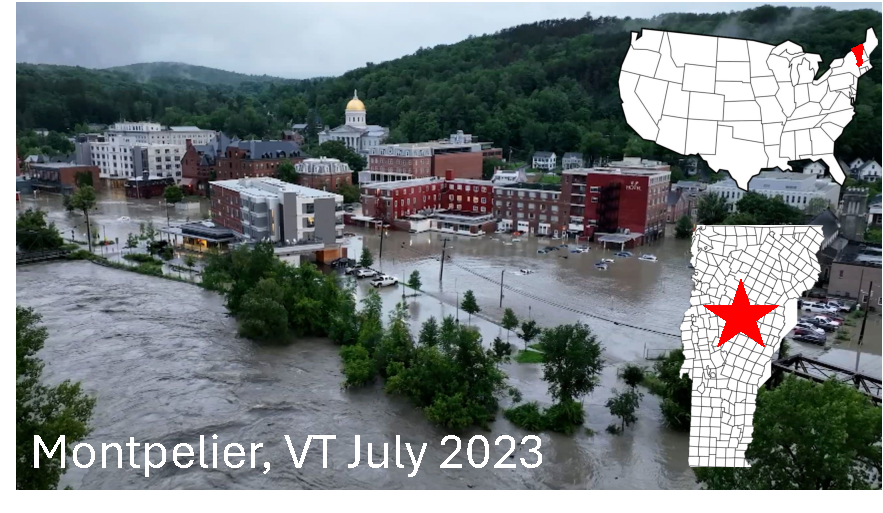
\includegraphics[width=0.38\textwidth]{images/vt.pdf}
\captionsetup{justification=centering,singlelinecheck=false,font=small}
\vspace{-0.9cm}
\caption{Montpelier during the July 2023 flood.}
\label{fig:vt}
\vspace{-0.3cm}
\end{wrapfigure}
\normalsize
Montpelier, Vermont's capital, sustained catastrophic flooding in July 2023
(80\% of its National Register Historic District damaged) and again in 2024, one
of over 45 such events since 1900 at the Winooski/North Branch confluence.
Its downtown core of 19th-century load-bearing masonry, largely pre-dating the
1933 ANSI code, is this proposal's pre-code archetype, with moderate institutional
capacity (emergency manager, SHPO support, planning department) but no
hydrodynamic simulation infrastructure.
The framework transfers to any municipality meeting four conditions, specifically riverine
flooding with building-level standing water persisting roughly five or more days;
pre-1940 construction as a meaningful share of the flood-exposed inventory; no
sustained in-house hydraulic modeling capacity; and USGS gauge coverage on the
primary watershed.
The first condition is defined on standing-water persistence in the building stock,
not on the shorter river-stage exceedance (Preliminary Results below). It is this
slow local drainage, not the river crest, that drives duration-governed masonry
degradation and that the mass balance model targets.
% resolved 2026-07-22: five-or-more-day threshold kept but explicitly redefined on building-level standing water rather than river stage, so the 28-hour flood-stage exceedance in the 2023 gauge record is not a counterexample to the scope condition.

\vspace{-10pt}
\subsection{Preliminary results: SAR building-level data, Montpelier 2023 and 2024}

SAR imagery captures flood extent through cloud cover and at night, when optical imagery fails. Open Sentinel-1 (C-band, ~10\,m resolution) and commercial ICEYE (X-band, $<$1\,m resolution) both cover the two Vermont events at the meter-scale, few-hour cadence this framework requires (Subtask~1.1).
In particular, ICEYE commercial SAR provides building-level flood depth and inundation maps fusing SAR amplitude imagery with LIDAR and water gauge measurements, at revisit cadences as fine as six hours during dense acquisition sequences, across the inundation and recovery period of both Montpelier flood events.
% CHRISTELLE: CONFIRM THE ACTUAL 2023/2024 SCENE CADENCE (WAITING ON FILE LIST, ITEM 4 IN FINDINGS.MD). ALSO: UNCERTAINTY OF FLOOD LEVEL -- KATIE/ICEYE INPUT? OTHER CAVEATS?
Through an NDA data access agreement, ICEYE data for 271 downtown pre-code masonry buildings, each with ICEYE-measured duration, peak depth, and field-recorded damage state, will be analyzed for both the 2023 and 2024 events (Subtask~1.1).
% see with ICEYE what text they want us to add and I think your preliminary screenshots are sufficient for the proposal but we should ask them if OK to include or if they prefer us to include something else with their logo super visible etc. TODO 
The 271-building dataset constitutes the empirical foundation for fragility surface calibration (2023) and held-out validation (2024); the 2024 data is not used in any model fitting (Fig.~\ref{fig:iceye}).

\begin{figure}[h]
\vspace{-0.2cm}
\centering
\begin{subfigure}[b]{0.48\textwidth}
  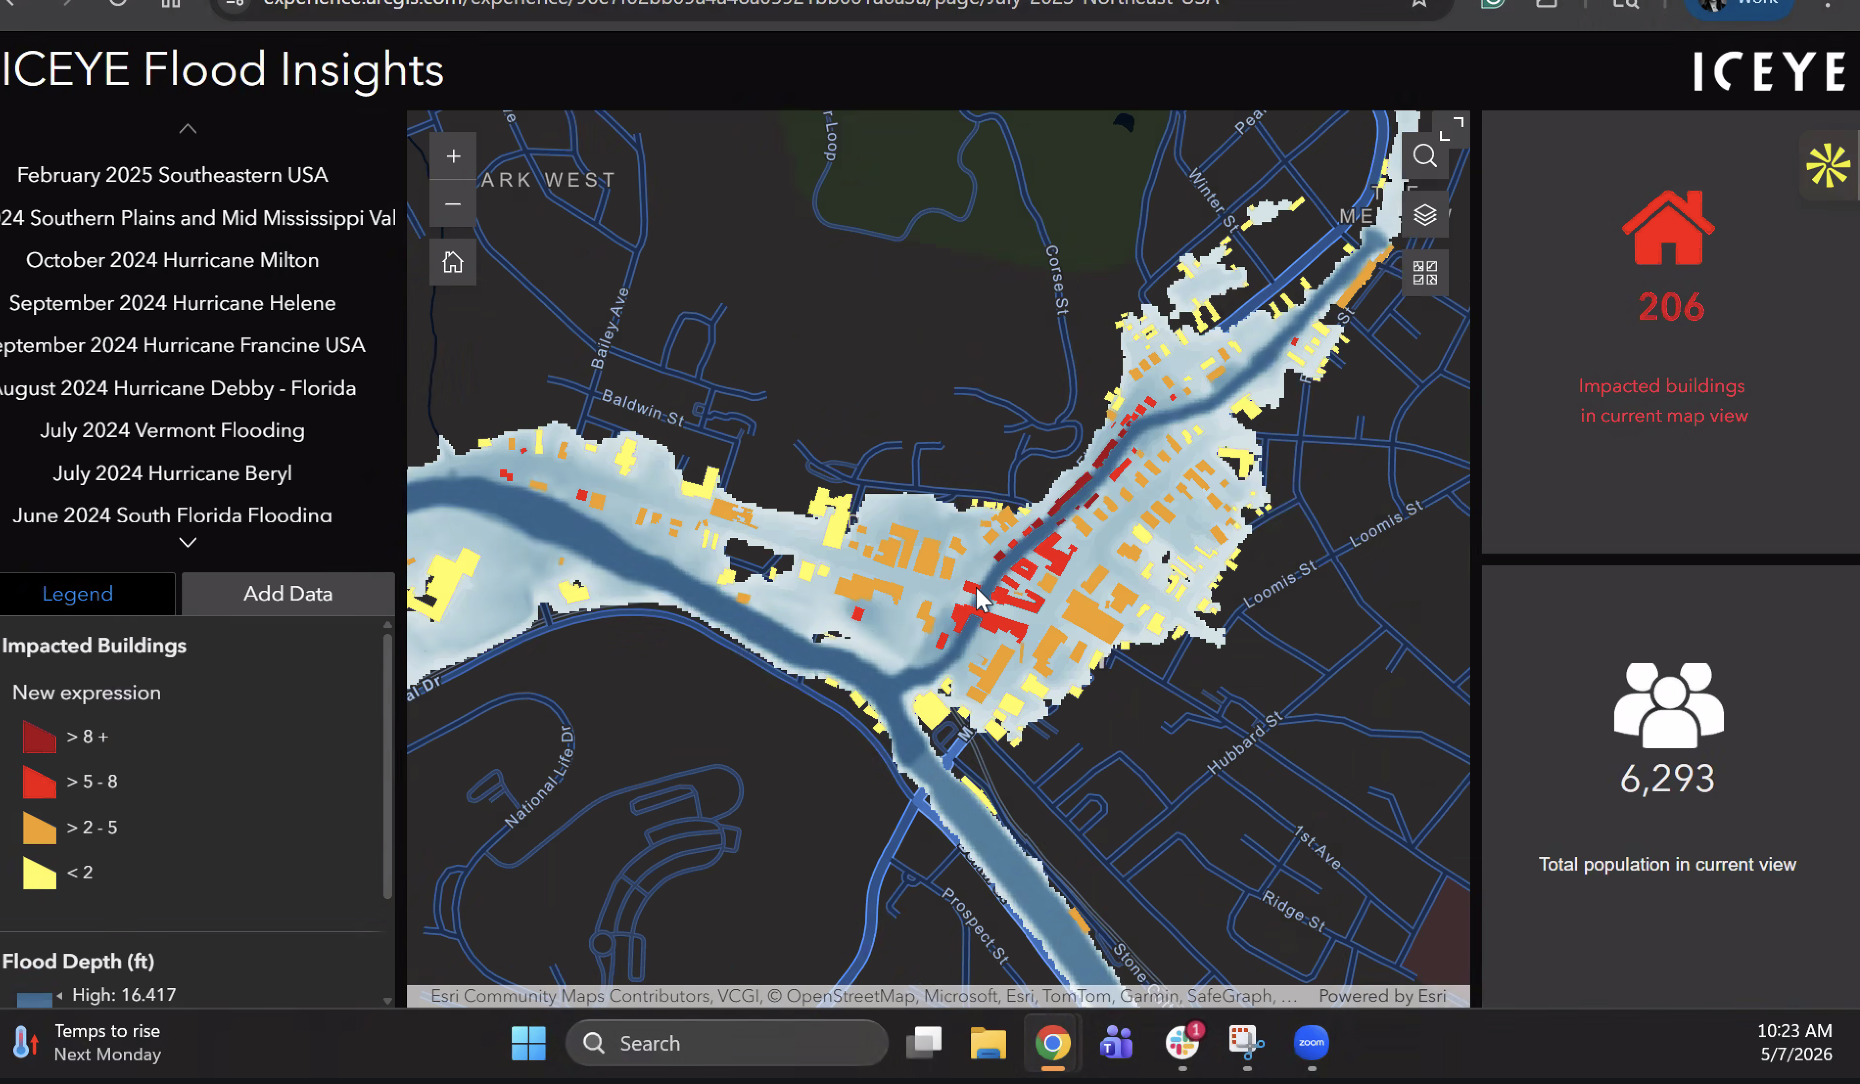
\includegraphics[width=\textwidth]{images/2023.png}
  \captionsetup{font=small}
  \caption{July 2023 (calibration event)}
  \label{fig:iceye_2023}
\end{subfigure}
\hfill
\begin{subfigure}[b]{0.48\textwidth}
  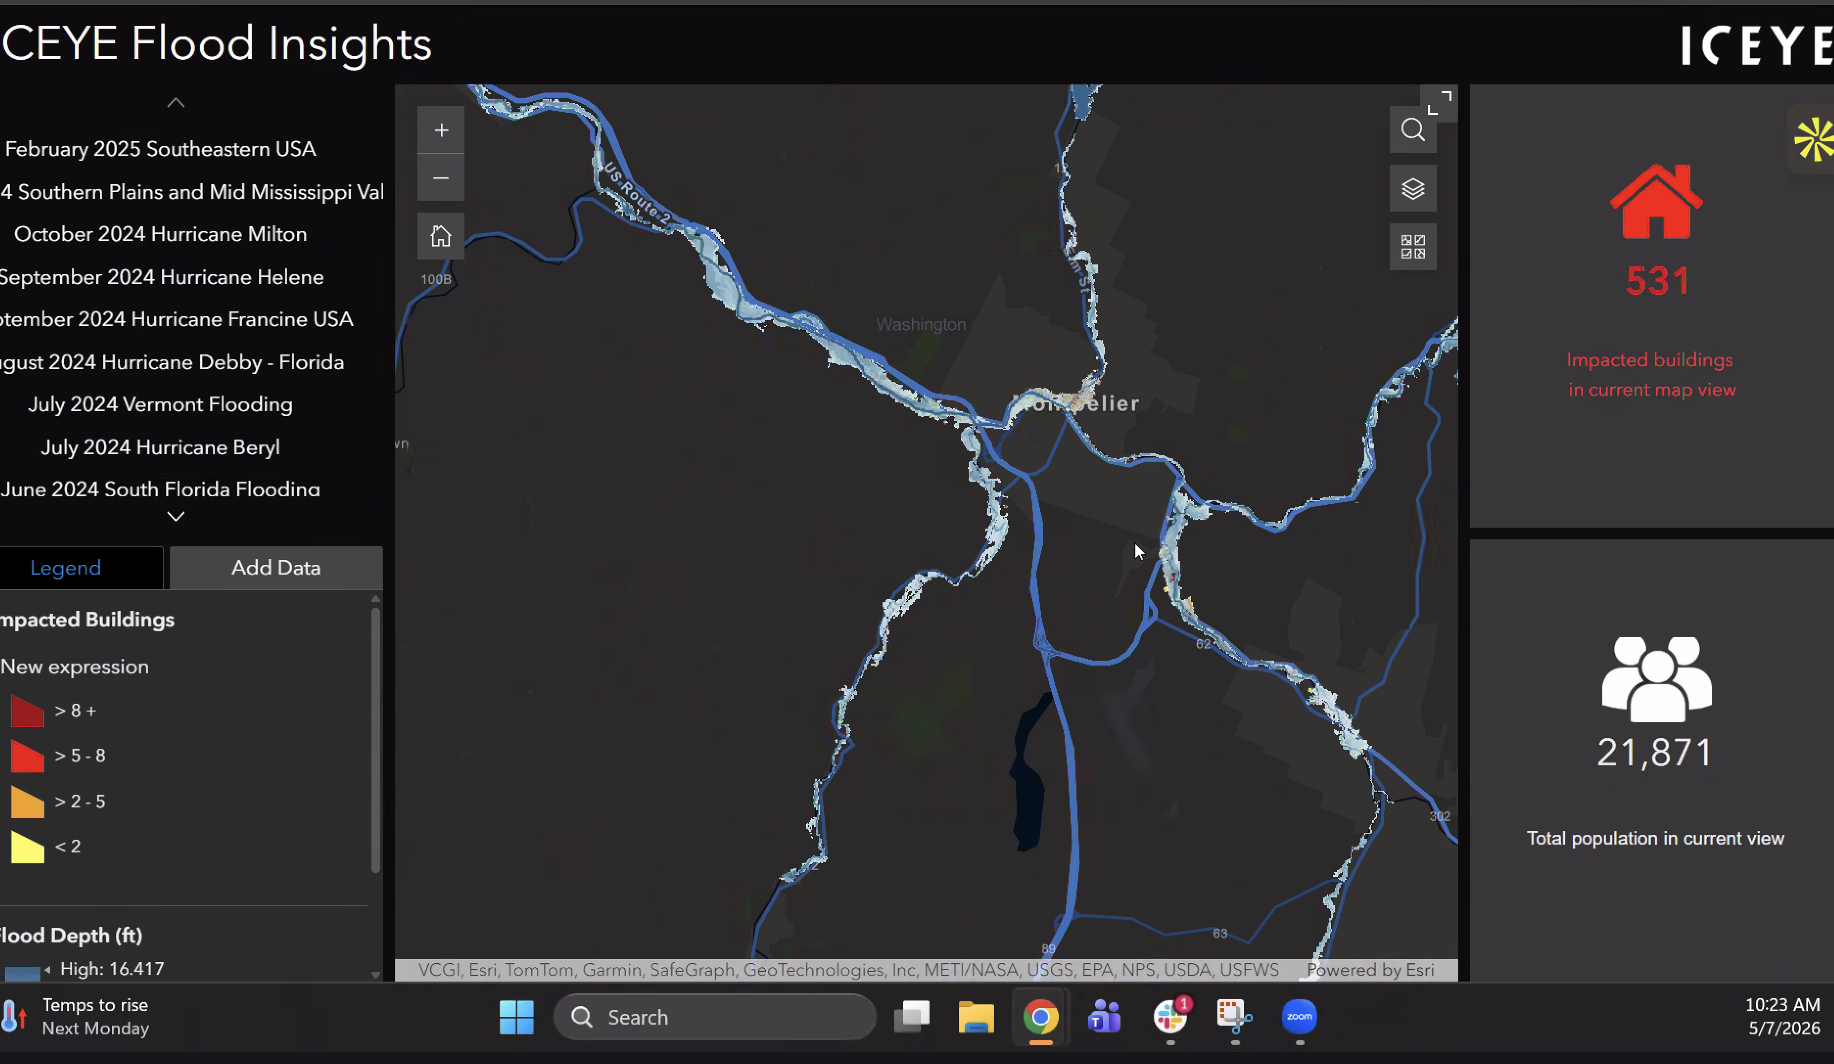
\includegraphics[width=\textwidth]{images/2024.png}
  \captionsetup{font=small}
  \caption{July 2024 (held-out validation event)}
  \label{fig:iceye_2024}
\end{subfigure}
\captionsetup{font=small}
\vspace{-0.3cm}
\caption{\hl{\textbf{CHECK WITH CHRISTELLE WHETHER THESE FIGURES ARE OK TO USE OR IF ICEYE PREFERS DIFFERENT ONES.}} ICEYE building-level flood depth, Montpelier downtown core, for both
study events. Building footprints are colored by peak inundation depth (yellow:
$<$2\,ft; orange: 2--5\,ft; red: 5--8\,ft; dark red: $>$8\,ft). Duration
brackets, as fine as six hours between successive overpasses, were extracted
separately for all 271 buildings across both events (Subtask~1.1).}
\label{fig:iceye}
\vspace{-0.3cm}
\end{figure}

% CHRISTELLE: ADD 2-3 SENTENCES DESCRIBING THE ICEYE PROCESSING PIPELINE AND ANY FLAGS ON THE DURATION AND DEPTH MEASUREMENTS.
%
% becca: get the correct figures from company for the full proposal, prob need two panels at the same zoom level: one showing 2023 downtown core (calibration event) and one showing 2024 (held-out validation event).

\subsection{Preliminary results: field damage assessment, Montpelier 2023}
PI Napolitano's team conducted a field damage assessment of the 271 downtown
masonry buildings before the July 2024 event, so the recorded states reflect
2023 damage only and the 2024 event remains fully held out. Damage states were
assigned from combined field inspection, city records, and owner reports using
three ordered states: no damage, cosmetic damage (e.g.\ water staining, minor
plaster loss), and structural damage (e.g.\ mortar deterioration, masonry
cracking, foundation compromise). The majority of buildings sustained damage,
consistent with the event severity (80\% of the National Register Historic District
affected). The three-state ordinal classification provides the resolution needed
for duration-dependent fragility surface calibration in Subtask~1.4.
Each of the 271 buildings in the ICEYE dataset (Fig.~\ref{fig:iceye}) carries
a field-assigned damage state on this three-level scale, paired building by
building with ICEYE-measured depth and duration. Approximately 75 sustained no
damage, 120 cosmetic damage, and 76 structural damage.
% becca: VERIFY THESE COUNTS AGAINST ACTUAL FIELD DATA — estimated from ICEYE depth distribution.

\subsection{Preliminary results: Winooski watershed drainage timescale}
To test whether the mass balance timescale is recoverable from free gauge data at
fragility-model accuracy, we ran a recession analysis of USGS gauge 04286000
(Winooski River at Montpelier; 397\,mi\textsuperscript{2}) for both events using
15-minute discharge records (Fig.~\ref{fig:recession}).
Three observations anchor the research plan.
First, the watershed-scale timescale (37--45\,h across both events) is stable, at the
day-to-multi-day order masonry degradation operates on, and recoverable from the
gauge record alone; Subtask~1.2 disaggregates this quantity to sub-basin scale
from national GIS layers.
Second, the 2023 recession departs from a single exponential beyond roughly
60 hours, consistent with a channel-to-storage transition
in which standing water in low-lying sub-basins outlasts the river recession, motivating
sub-basin $\hat{\tau}_k$ estimates over one watershed constant.
Third, the events differ nearly twofold in peak magnitude, and the 2024 peak
stage stayed below minor flood stage even as downtown parcels took
water, so the 2023-calibrated, 2024-validated design tests transfer across event
magnitudes rather than replicating one event size.
The standing-water distinction is concrete. The
2023 gauge stood above NWS minor flood stage for 28 hours, yet building interiors
were still being pumped days later. The
State Street office complex took four to five days to clear
\cite{vermontpublic2023stateflood}, the Montpelier High School basement five to
six days \cite{vtdigger2023schools}, and downtown streets roughly two days
\cite{vermontpublic2023recede}.
Building-level standing water, the quantity $T_i$ the framework models, thus
outlasted river-stage exceedance by days in 2023, the separation sub-basin
timescales $\hat{\tau}_k$ are designed to capture.
A prototype stage-to-digital-elevation-model (DEM) projection (1\,m USGS 3DEP
terrain, gauge datum 499.87\,ft NAVD88) of the 2023 crest reproduces
river-corridor inundation but underpredicts the flooded core by 0.8 to 1.5\,m,
implying a water-surface slope of 0.6 to 1.0\,m/km, the single parameter the
2023 ICEYE depth field calibrates (Subtask~1.2).
% becca: images/stage_dem_depth.pdf (depth map with gauge and landmarks marked) exists if you want a figure for the stage-to-DEM prototype; left out of the text for space. Script: analysis/stage_to_dem.py, writeup: analysis/stage_dem.md.
% maggie: this is a first-pass PI recession analysis (script in analysis/winooski_recession.py) so you have real numbers to build from. Your call on: sub-basin delineation and a sub-basin map, the functional form for tau_k_hat, and whether to redo the fit with your preferred recession method. Replace or extend freely; the figure regenerates from the script.

\begin{figure}[h]
\vspace{-0.2cm}
\centering
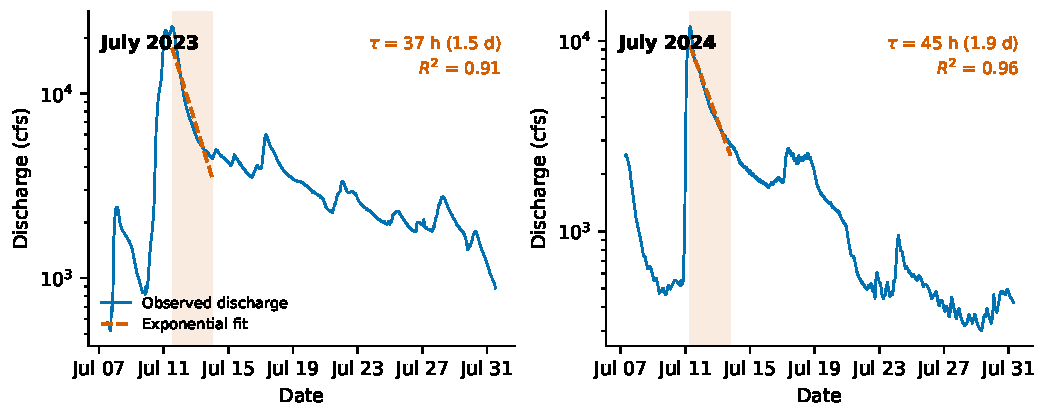
\includegraphics[width=\textwidth]{images/winooski_recession.pdf}
\captionsetup{font=small}
\vspace{-0.5cm}
\caption{Recession analysis of USGS gauge 04286000 (Winooski River at
Montpelier), July 2023 (left) and July 2024 (right), from 15-minute discharge
records. Dashed lines show exponential fits over the shaded 60-hour windows:
$\tau = 37$\,h ($R^2 = 0.91$) and $\tau = 45$\,h ($R^2 = 0.96$).}
\label{fig:recession}
\vspace{-0.3cm}
\end{figure}

% ============================================================
%  RESEARCH PLAN
% ============================================================

\section{Research plan}
RO1 (Napolitano, Wauthier, Busse) addresses RQ1 through five subtasks (1.1 to 1.5); RO2 (Napolitano with all PIs) addresses RQ2 through five subtasks (2.1 to 2.5). Together the two objectives close the loop end to end, operating at three timescales rather than through continuous automated actuation, spanned by two interface modes. Hours before a flood peak, NOAA forecasts drive pre-storm resource staging; over years, retrofit decisions feed back through the $\hat{\tau}_k$ and fragility updates of Subtask~2.4, changing the flood behavior the system models next (both via Plan/Forecast mode). After each event, community priors and the error model update from what the flood revealed (Update Model mode). Human decisions are the actuators at every timescale, making the community a functional component of the control loop rather than a recipient of its outputs. The research questions emerged directly from PI Napolitano's post-2023 Montpelier engagement. Community partners asked where limited flood-mitigation dollars belong, and that question defined the decision problem.

% ── RO1 BOX ──────────────────────────────────────────────────────────────────
\begin{tcolorbox}[colback=mycmykcolor,colframe=black,boxrule=1pt,coltext=black,
  left=1mm,right=1mm,top=1mm,bottom=1mm]
\textbf{Research Objective 1 (RO1, leads: Napolitano, Wauthier, and Busse):
Develop and validate a closed-loop CPS coupling a GIS-parameterizable mass balance
model with community knowledge in a Bayesian framework and duration-dependent
fragility surfaces for pre-code masonry archetypes, and establish whether the system
is decision-adequate for retrofit allocation and pre-storm resource staging without
hydraulic simulation, calibrated on Montpelier 2023 and validated on the held-out
2024 event.}
\end{tcolorbox}

RO1 builds the first three capabilities identified in the state of the art.
Subtask~1.1 processes ICEYE SAR imagery (with open Sentinel-1 for flood-extent
context) into the interval-censored duration brackets and peak depths that
calibrate the framework. Subtask~1.2 develops the GIS-parameterizable mass balance
model that estimates how long water stays. Subtask~1.3 fuses mass balance
predictions with community knowledge priors in a Bayesian framework, where
community knowledge enters as the building-level adjustment
$\delta_i^{\mathrm{comm}}$ supplied and characterized by RO2. Subtask~1.4
translates the resulting duration and depth estimates into damage through
duration-dependent fragility surfaces for pre-code masonry.
ICEYE provides one-time calibration data for the error model and fragility
surface; the operational system runs entirely on USGS gauge data and NOAA
precipitation, which are free and nationally available.
Subtask~1.5 validates the full RO1 system against the 2024 held-out event and
characterizes decision-adequacy for scenario-based retrofit ranking and forecast-driven staging.

\textbf{Subtask 1.1: SAR Data Processing, Interpretation, and Likelihood Characterization
(lead: Wauthier).}
Subtasks~1.1 and~1.2 run in parallel in Year~1 and are independent until both feed the Bayesian fusion framework in Subtask~1.3.
PI Wauthier processes ICEYE commercial SAR data for the 271 downtown Montpelier buildings across both flood events, extracting building-level peak depth and per-overpass wet/dry status, and validating building footprint attribution against ground-referenced building inventory.
Because duration is inferred from wet/dry status across successive overpasses, each building's inundation duration is delivered not as a point value but as a bracket between the last overpass observed wet and the first observed dry, with bracket width set by the acquired revisit cadence (as fine as six hours where the acquisition sequence is dense); this bracket is carried through the framework as an explicit measurement interval rather than collapsed to a false point estimate.
The key scientific outputs of this subtask are the per-building duration brackets and peak depths for both events, together with per-scene wet/dry classification error rates; once Subtask~1.2 delivers $\hat{\tau}_k$ estimates, comparing mass balance predictions against the 2023 brackets calibrates the building-scale error variance $\sigma_{\mathrm{MB}}^2$ of the GIS-parameterized model in Subtask~1.3.
Preliminary cadence simulation shows that scenes spread across the multi-day drainage window carry substantially more calibration information than scenes clustered near the peak, and this criterion prioritizes which acquisitions are processed.
Open Sentinel-1 imagery is processed for both events for broader flood-extent context; at ~10\,m resolution it cannot resolve individual downtown buildings, so it supports cross-checking of the ICEYE classifications rather than feeding the building-level likelihood.

\hl{\textbf{CHRISTELLE: ADD ICEYE PROCESSING PIPELINE DESCRIPTION AND DEPTH/DURATION MEASUREMENT FLAGS. CONFIRM SCENE CADENCE FOR BOTH EVENTS.}}

\textbf{Subtask 1.2: GIS-Parameterizable Mass Balance and Depth Projection (lead: Busse).}
Subtask~1.2 develops two complementary models, both parameterized entirely from
national GIS layers, a mass balance model that estimates drainage timescale
$\hat{\tau}_k$ per sub-basin, and a stage-to-DEM projection that estimates
building-level peak depth $d_i$.
PI Busse develops the mass balance model for the Winooski watershed above
Montpelier, estimating $\hat{\tau}_k$ for each drainage sub-basin from watershed delineation and contributing
area from USGS 3DEP and NHD StreamStats, effective impervious fraction from NLCD,
soil infiltration rates from SSURGO, and real-time discharge from USGS station
04286000.
% corrected 2026-07-22: the tex previously said 04288000, which is the Mad River near Moretown; 04286000 is the Winooski River at Montpelier (verified against the USGS NWIS site record).
Each sub-basin is modeled as a linear reservoir, the storage-discharge form whose
signature is the exponential recession observed in the preliminary gauge analysis:
\begin{equation}\label{eq:tau}
  \frac{dS_k}{dt} \;=\; I_k(t) \;-\; Q_k,
  \qquad
  Q_k \;=\; C_k\,\frac{S_k}{S_k^{\mathrm{max}}} \;=\; \frac{S_k}{\hat{\tau}_k},
  \qquad
  \hat{\tau}_k \;=\; \frac{S_k^{\mathrm{max}}}{C_k}
\end{equation}
where $S_k$ is stored floodwater volume in sub-basin $k$, $I_k(t)$ is inflow from
precipitation and upstream routing, $S_k^{\mathrm{max}}$ is the storage capacity
of the sub-basin's low-lying terrain from 3DEP, and $C_k$ is its effective
conveyance and infiltration capacity from NHD channel properties, NLCD
imperviousness, and SSURGO infiltration rates. Outflow is closed as a linear
function of fractional storage, $Q_k = C_k\,S_k/S_k^{\mathrm{max}}$, so once
inflow subsides the storage decays exponentially and $\hat{\tau}_k =
S_k^{\mathrm{max}}/C_k$ is the genuine e-folding recession constant, consistent
with the exponential falling limbs fit in the preliminary gauge analysis
($\hat{\tau} = 37$ and $45$~h).
% MAGGIE: LINEAR-RESERVOIR FORM WITH FRACTIONAL-STORAGE OUTFLOW CLOSURE (Q_K = C_K S_K / S_K^MAX) COMMITTED HERE. REPLACE WITH YOUR PREFERRED TAU_K_HAT FORMULATION IF DIFFERENT, AND ADJUST THE CLOSURE AND PARAMETERIZATION LANGUAGE TO MATCH.
The drainage timescale $\hat{\tau}_k$ represents the expected duration of standing
water under gravitational drainage and serves as the physically grounded prior mean
on inundation duration; the model is designed so that any municipality with a USGS
gauge ID and access to standard national GIS layers can parameterize it without
field data collection.
Sub-basins are delineated from 3DEP flow paths at the scale where storage and
conveyance properties are resolvable from national layers, on the order of ten to
twenty sub-basins across the flood-exposed core; preliminary terrain-partition
sensitivity analysis indicates this granularity sits
inside the plateau where finer partitioning adds degrees of freedom without
adding explained building-level variation.
Building counts per sub-basin are strongly skewed, from a dominant main-corridor sub-basin holding tens of buildings to single-building tributary sub-basins; the model is deliberately lumped at this scale, with per-building variation carried by the community adjustment $\delta_i^{\mathrm{comm}}$ and the error variance rather than by finer hydraulics.
Inundation duration at building $i$ in sub-basin $k$ is modeled as:
\begin{equation}\label{eq:prior}
  T_i \sim \operatorname{LogNormal}(\mu_i,\; \sigma_{\mathrm{MB}}^2)
\end{equation}
where the log-scale prior mean is:
\begin{equation}\label{eq:mu}
  \mu_i \;=\; \log \hat{\tau}_k \;+\; \delta_i^{\mathrm{comm}}
\end{equation}
$\hat{\tau}_k$ is the mass balance drainage timescale for sub-basin $k$ and
$\sigma_{\mathrm{MB}}^2$ is the building-scale error variance of the
GIS-parameterized mass balance. It absorbs both residual local drainage
variability and the model's systematic limitations at building scale, so that
all model error lives on the prior side of the framework rather than being
attributed to the sensing data.
$\sigma_{\mathrm{MB}}^2$ is a cross-sectional quantity, the building-to-building
spread of durations within a single event, and it is estimated from the 2023 SAR
brackets in Subtask~1.3, with the gauge record supplying only a weak regularizing
anchor. A recession analysis of fifteen well-fit flood events in the gauge's
1990 to 2026 instantaneous record gives an
event-to-event variability of the watershed timescale,
$\sigma_{\mathrm{event}} = \mathrm{sd}(\ln \hat{\tau}) = 0.30$. This is a
storm-to-storm variability of one aggregate parameter, physically distinct from
the within-event, building-to-building heterogeneity that $\sigma_{\mathrm{MB}}$
measures, so $\sigma_{\mathrm{event}}$ is not used as $\sigma_{\mathrm{MB}}$
itself but only as an order-of-magnitude anchor keeping the Subtask~1.3
calibration in a plausible range; preliminary sensitivity analysis confirms the
calibration is robust to mis-scaling of this anchor, with a factor-of-two
mis-scaling moving the calibrated $\sigma_{\mathrm{MB}}$ by less than 0.01 under
realistic acquisition cadences, and the 271 brackets carrying over 80 percent of
the identifying weight even with a single usable post-peak scene.
Subtask~1.2 delivers the GIS-only prior, setting $\delta_i^{\mathrm{comm}} = 0$
gives the baseline model parameterized entirely from national GIS layers, which
constitutes both the operational system for transfer communities and the comparison
baseline for RQ2.
The building-level adjustment $\delta_i^{\mathrm{comm}}$, elicited from community
knowledge in Subtask~2.1 (locally known drainage obstructions, historically slow
routes, anomalous building conditions), augments this baseline in Subtask~1.3;
community knowledge improves the system but is not required to run it.
The LogNormal family is appropriate because duration is strictly positive and right-skewed and keeps the log-scale consistency used by the Subtask~1.3 bracket likelihood. All duration quantities are conditional on inundation. $T_i$ is the standing-water duration at building $i$ given that it floods, and the Subtask~1.3 error model characterizes duration error, not flood/no-flood classification.
Whether a building floods, and to what peak depth, is supplied by a second,
deliberately simple computational component, a stage-to-DEM mapping that projects
gauge crest stage onto the USGS 3DEP terrain model along a reach-scale
water-surface slope:
\begin{equation}\label{eq:stagedem}
  d_i \;=\; \max\bigl\{\,0,\; (s_g + \beta\, x_i) - z_i \bigr\}
\end{equation}
where $s_g$ is the crest water-surface elevation at the gauge, $\beta$ is the
reach-scale water-surface slope, $x_i$ is the along-channel distance of building
$i$ upstream of the gauge, and $z_i$ is the building's ground elevation from
3DEP; a building is predicted inundated where $d_i > 0$, so the same mapping
supplies both building-level peak depth and the inundation extent.
In Plan/Forecast mode the projection takes either a scenario crest stage (for example a recurrence of the 2023 crest) or the NWS river-stage forecast for the gauge.
The 2023 ICEYE depth measurements calibrate the mapping's water-surface slope
$\beta$ and bound its building-level error in
the same way the 2023 duration brackets calibrate the mass balance error, and that
calibrated error defines a distribution over $d_i$ rather than a single point
value; the depth input required by the fragility surface of Subtask~1.4 in every
operational mode is produced by this component, not by the mass balance model.
A single reach-scale $\beta$ is appropriate here even though the duration model
resolves ten to twenty sub-basins. The flood water surface along the downtown
reach is a smooth, hydraulically connected profile, a property of the reach as a
whole rather than of any individual sub-basin, and preliminary slope sensitivity
analysis bounds the admissible range of $\beta$ from
documented 2023 flood outcomes ahead of the ICEYE-based calibration.
For pre-storm prediction, NOAA forecast precipitation replaces observed discharge
as the model input; forecast uncertainty is propagated through the mass balance to
produce appropriately wider credible intervals on predicted duration.

\hl{\textbf{MAGGIE: CONFIRM OR REPLACE TAU FORMULATION. PROVIDE SUB-BASIN DISCRETIZATION AND AMC HANDLING (SEE COMMENTS IN SOURCE).}}

% MAGGIE: EQ:TAU COMMITS TO TAU_K_HAT = S_K^MAX / C_K. CONFIRM OR REPLACE. STILL NEEDED: SPATIAL DISCRETIZATION (APPROXIMATE SUB-BASIN SIZE), AND WHETHER THIS USES AN EXISTING WINOOSKI MODEL OR REQUIRES NEW DEVELOPMENT.
%
% MAGGIE -- IMPORTANT FOR PRE-STORM MODE: (1) DOES THE MODEL INCLUDE AN ANTECEDENT MOISTURE
% CONDITION (AMC) INPUT (E.G., AMC-I/II/III FROM TR-55, OR CONTINUOUS SOIL MOISTURE FROM
% SSURGO + PRIOR PRECIP)? (2) HOW IS AMC ESTIMATED OPERATIONALLY BEFORE A STORM (NOAA QPF
% HISTORY? USGS SOIL MOISTURE NETWORK?)? (3) HOW MUCH DOES TAU_K_HAT VARY BETWEEN DRY AND
% SATURATED CONDITIONS? IF LARGE AND UNCERTAIN, PRE-STORM CREDIBLE INTERVALS MAY LIMIT
% ACTIONABILITY AND WE SHOULD NARROW THE PRE-STORM CLAIM. VERIFIED REFS IN BIBLIO.BIB:
% USDASCS1986TR55 (TR-55 AMC CLASSES), KIM2019ASSESSMENT (AMC EFFECT, NAPA RIVER).
% note 2026-07-22 (PI): partial empirical answer now in analysis/historical_tau.md -- across 15 well-fit events (1990-2026) tau ranges 36-96 h, correlates with normalized pre-event baseflow (r=0.59, ~+33 h shift dry-to-wet). Wetter antecedent = SLOWER recession. Pre-event baseflow is an operational AMC proxy from the same gauge. Maggie's question about the model formulation still stands.

\textbf{Subtask 1.3: Bayesian Fusion Framework (leads: Napolitano, Wauthier,
and Busse).}
Subtask~1.3 formulates building-level inundation duration as a state-estimation
problem, recovering a latent physical quantity from two information sources with
two distinct error structures. The mass balance model, whose building-scale
prediction error is
carried by the prior variance $\sigma_{\mathrm{MB}}^2$, and the SAR observations,
whose uncertainty is a sampling property of the acquisition schedule rather than
an instrument noise floor.
A building's inundation duration is never observed directly. Each SAR overpass
records only whether the building is inundated at that instant, so the
observations constrain the true duration to a bracket $T_i \in [L_i, U_i]$, where $L_i$ is the elapsed time to the last overpass at which building $i$ is
observed inundated and $U_i$ the elapsed time to the first overpass at which it
is observed dry; the bracket width is the revisit spacing of the acquired scenes.
A building still observed wet at the final acquired scene is right-censored, with
$U_i$ unbounded; the same survival machinery applies, with likelihood
$1 - \Phi\!\left((\ln L_i - \mu_i)/\sigma_{\mathrm{MB}}\right)$.
The likelihood of the observed wet/dry sequence is the prior probability mass on
the bracket,
$\Phi\!\left(\tfrac{\ln U_i - \mu_i}{\sigma_{\mathrm{MB}}}\right) -
 \Phi\!\left(\tfrac{\ln L_i - \mu_i}{\sigma_{\mathrm{MB}}}\right)$,
and the posterior is the prior truncated to it:
\begin{equation}\label{eq:posterior}
  T_i \mid [L_i, U_i] \;\sim\;
  \operatorname{LogNormal}(\mu_i,\; \sigma_{\mathrm{MB}}^2)
  \ \text{truncated to}\ [L_i,\; U_i]
\end{equation}
This interval-censored formulation treats the SAR observations honestly, with a
dense acquisition sequence the brackets are hours wide and the posterior is
sharply localized; with sparse acquisitions the brackets widen and the SAR data
constrain the posterior only weakly.
Per-scene wet/dry classification error $\epsilon_j$, characterized by PI Wauthier
in Subtask~1.1, generalizes the hard bracket to a product of per-overpass
observation probabilities,
\begin{equation}\label{eq:softbracket}
  p(\bm{y}_i \mid T_i) \;=\; \prod_{j}
  (1-\epsilon_j)^{\,\mathbf{1}\{y_{ij} = \mathbf{1}\{t_j < T_i\}\}}\;
  \epsilon_j^{\,\mathbf{1}\{y_{ij} \neq \mathbf{1}\{t_j < T_i\}\}}
\end{equation}
where $y_{ij}$ is the wet/dry classification of building $i$ at overpass time
$t_j$; as $\epsilon_j \to 0$ this recovers the hard bracket $T_i \in [L_i, U_i]$, so classification error softens the truncation
boundaries without changing the structure.
$\sigma_{\mathrm{MB}}^2$ is calibrated on the 2023 event by maximum likelihood
over the 271 interval-censored observations with the GIS-only prior
($\delta_i^{\mathrm{comm}} = 0$), using the classification-error-softened
likelihood of Equation~\eqref{eq:softbracket} with the per-scene error rates
$\epsilon_j$ characterized in Subtask~1.1; this reduces to the hard-bracket
survival likelihood where those error rates are small. Working on the log scale
maintains dimensional consistency with the LogNormal prior and keeps all duration
quantities strictly positive.
The $\sigma_{\mathrm{event}}$ anchor centers a weak regularizing prior on
$\sigma_{\mathrm{MB}}$ in this calibration, where the acquired brackets are wide,
the censored likelihood constrains $\sigma_{\mathrm{MB}}^2$ only weakly and the
estimate falls back toward the anchor rather than becoming unidentified, and the
detectability statements reported in Subtask~2.3 make explicit what the acquired
cadence can and cannot resolve.
Preliminary simulation quantifies this graceful degradation. Across acquisition cadences from uniform
six-hourly coverage down to a single usable post-peak scene,
$\sigma_{\mathrm{MB}}$ remains identified with estimation uncertainty that grows
continuously rather than collapsing, and the regularizing prior narrows the
estimate at every cadence at a bias cost bounded by the anchor's own scale.
Within this framework, the fusion that defines the computational core is between the
physically grounded mass balance prior and the community knowledge adjustments
$\delta_i^{\mathrm{comm}}$ of Equation~\eqref{eq:mu}; the SAR brackets calibrate the error
model on 2023 and adjudicate between prior variants on 2024, but the operational
system never depends on them.
Posteriors are computed independently per building; this is a simplification of
the within-sub-basin spatial correlation of inundation durations, and its practical
consequence is that portfolio-level uncertainty across neighboring buildings in the
same sub-basin may be marginally underestimated; for the retrofit ranking decisions
this proposal targets, priority rankings are robust to this approximation.
For operational deployment without SAR imagery, the predictive distribution is
the prior with the adjustment uncertainty folded in, $T_i \sim
\operatorname{LogNormal}(\mu_i,\; \sigma_{\mathrm{MB}}^2 + P_i)$, where $P_i$ is
the tracked variance of the community adjustment from Subtask~2.4 and is zero in
the GIS-only baseline; this variance carries the full building-scale error of
the GIS-parameterized system together with the uncertainty of any elicited
adjustment, the honest predictive uncertainty of the system when operating on
free data alone.
The 2024 Montpelier event is the held-out test. The calibrated framework, with
all parameters fixed from 2023, is applied to 2024 gauge and NOAA forecast data
and scored against the independently acquired 2024 SAR duration brackets.

\textbf{Subtask 1.4: Duration-Dependent Fragility Surface Development
(lead: Napolitano).}
Subtask~1.4 uses the processed ICEYE duration and depth for all 271 buildings (Subtask~1.1), runs in parallel with Subtasks~1.2 and~1.3, and does not depend on the mass balance model.
Duration and peak depth are correlated in the Montpelier 2023 data, motivating a two-component approach that separates the duration effect physically before fitting it statistically.
The \textit{physical component} sets the functional form of the duration effect from
published masonry degradation mechanisms (mortar softening, brick saturation,
rising damp), independently of observational confounding.
The \textit{empirical component} calibrates the surface parameters from the 2023
field damage observations, using ICEYE-measured depth and interval-censored
duration brackets as covariates for all 271 buildings; consistent with
Subtask~1.3, duration enters as its bracket, with estimation integrating over
each building's bracket by Monte Carlo sampling from the truncated posterior
of Equation~\eqref{eq:posterior}.
The fragility surface for damage state $ds$ takes the form:
\begin{equation}\label{eq:fragility}
  P(DS \geq ds \mid T_i,\; d_i) \;=\; \Phi\!\left(
    \frac{\ln T_i - \lambda_{0,ds} - \gamma \ln d_i}{\zeta}\right)
\end{equation}
where $T_i$ is inundation duration (hours), $d_i$ is peak inundation depth (m),
$\lambda_{0,ds}$ is the log-scale median duration capacity for damage state $ds$
at reference depth, $\gamma$ is the shared depth sensitivity (depth shifts the
threshold at which duration governs damage), $\zeta$ is the shared log-standard
deviation of capacity, and $\Phi$ is the standard normal cumulative distribution
function. With the three field-observed damage states (no damage, cosmetic,
structural), $ds \in \{1,2\}$ yields two exceedance curves,
$P(DS \geq \text{cosmetic})$ and $P(DS \geq \text{structural})$. The thresholds
are constrained to be ordered, $\lambda_{0,1} < \lambda_{0,2}$, while
$\gamma$ and $\zeta$ are shared across damage states, so the exceedance curves are
horizontal translates of one another along the $\ln T_i$ axis and cannot cross at any $(T_i, d_i)$; their
successive differences therefore define a valid ordinal damage-state distribution
everywhere.
Estimation is Bayesian. Published saturation-strength and capillary-absorption
curves for historic brick and lime mortar
\cite{hall2009water,franzoni2015compressive,sathiparan2018effect} supply
informative priors, with $\lambda_{0,ds}$ and $\gamma$ centered at the
material-science-derived values and prior variances set from specimen-to-specimen
scatter, updated by the interval-censored 2023 field-damage likelihood. The
resulting posterior surface is applied unchanged to 2024 for held-out validation.
The claim under test is that duration adds explanatory power beyond depth alone.
Because duration and depth are collinear in the 271-building sample, this claim is
posed not as a naive coefficient $t$-test on the correlated data but as a
comparison of posterior predictive accuracy on held-out 2024 damage between the
bivariate model and a depth-only baseline. The Bayesian machinery makes both the
identification and the significance claim coherent. The informative priors on
$\lambda_{0,ds}$ and $\gamma$ carry the identification the collinear 2023
covariates cannot, so the posterior shrinks toward the physical anchor where the
empirical signal is weak and refines the anchored values in a genuinely
data-driven way where it is strong.
Duration-depth collinearity is quantified directly from the 2023 covariates.
The bivariate versus depth-only comparison uses the interval-censored log
predictive score of Equation~\eqref{eq:lps}, summed across buildings, on the
held-out 2024 event, consistent with the Bayesian framework used throughout.
The posterior duration distribution from Subtask~1.3 (Equation~\eqref{eq:posterior}) propagates through
Equation~\eqref{eq:fragility} by Monte Carlo integration, which samples $d_i$ jointly with $T_i$ from the
calibrated depth distribution, so both fragility covariates carry quantified uncertainty into the decision
interface and the resulting building-specific damage state probability distribution reflects the full
inferential uncertainty of the mass balance, the depth projection, and the likelihood. Preliminary
sensitivity analysis quantifies the relative contribution of
depth-projection error and duration-bracket width to this uncertainty. The split is cadence dependent,
with duration dominating where brackets are wide (depth error carries a median share of roughly four
percent under the on-file 2023 acquisition) and depth-projection error becoming the dominant remaining
source where dense six-hour brackets pin duration tightly, which is why both covariates carry propagated
uncertainty rather than depth being treated as exact.
The 271-building sample is predominantly load-bearing brick unreinforced masonry
(URM), with a small number of mixed brick-and-stone construction; together these
constitute the pre-code archetype the fragility surface targets.
% becca: confirm damage state definitions (ordinal levels if they exist, or binary) and distribution across the 271 buildings. Add damage map figure when ready.

\textbf{Subtask 1.5: System Validation (leads: all three PIs).}
Subtask~1.5 validates the full RO1 system against the 2024 held-out event for scenario-based retrofit ranking and forecast-driven staging, with all model parameters fixed from 2023 calibration.
Technical validation scores predictive duration distributions from the Bayesian
framework against the 2024 SAR duration brackets for all 271 buildings, reporting
the interval-censored log predictive score, empirical consistency of 90\% credible
intervals with the observed brackets (a well-calibrated system should have
approximately 90\% of brackets consistent with the corresponding intervals), and
root mean square error against bracket midpoints where the acquisition cadence
makes brackets tight; calibration in the strict
frequentist sense requires repeated experiments, and the 271-building 2024 dataset
constitutes one draw from the event distribution rather than independent trials,
so coverage assessment from a single event is limited; the design uses all 271
buildings as assessment units and multi-event calibration assessment is a target
for future work.
The interval-censored log predictive score for building $i$ is
\begin{equation}\label{eq:lps}
  \mathrm{ILS}_i \;=\; -\log\!\left[
    \Phi\!\left(\frac{\ln U_i - \tilde{\mu}_i}{\tilde{\sigma}_i}\right) -
    \Phi\!\left(\frac{\ln L_i - \tilde{\mu}_i}{\tilde{\sigma}_i}\right)\right]
\end{equation}
where $\tilde{\mu}_i$ and $\tilde{\sigma}_i$ are the predictive log-duration
parameters for building $i$ with all model components fixed from 2023; it is a
proper scoring rule under interval censoring, and the same score adjudicates the
prior variants compared in Subtask~2.3.
Damage state validation compares Equation~\eqref{eq:fragility} fragility surface predictions against
2024 field damage observations at building scale, using the posterior duration
distributions as input; the claim under test is that the duration-depth bivariate
model predicts 2024 damage states more accurately than a depth-only baseline fitted
on the same 2023 data.
Because 2024 was a smaller-magnitude event, the statistical power of this held-out
comparison depends on the damage variation the event actually produced; the
comparison is therefore reported alongside a cross-validated bivariate versus
depth-only comparison on the 2023 calibration data, and the 2024 result is stated
relative to the observed 2024 damage-state distribution rather than as an
unconditional significance claim.
Decision-adequacy validation assesses whether retrofit priority rankings from
Plan/Forecast mode align with independent rankings produced by community partners and
domain experts based on direct knowledge of 2024 damage outcomes. The expert panel
draws from the Association for Preservation Technology International Disaster
Response Initiative (APT DRI), a group of preservation and emergency management
professionals who work on historic disaster response and data curation, co-led by
PI Napolitano. Alignment is assessed by rank correlation, and systematic divergence
between model and expert rankings is treated as a finding requiring explanation
rather than suppression.
Forecast validation applies the framework retrospectively to the 2024 event
using NOAA quantitative precipitation forecast products at 24-, 48-, and 72-hour
lead times before the flood peak; predicted building-level inundation risk maps are
compared against SAR imagery products, and prediction accuracy is reported as a function
of lead time to characterize how forecast uncertainty degrades prediction
quality and what actionable lead time the system can reliably provide.
% becca: confirm that 2024 field damage observations will be available for the damage state comparison.

\textbf{Key outcomes:} RO1 produces three primary outputs: a validated Bayesian framework, with community knowledge entering as a structural calibration input, with characterized decision-adequacy for scenario-based retrofit ranking and forecast-driven staging (Subtasks~1.3 and~1.5); duration-dependent fragility surfaces for the pre-code masonry building stock (Subtask~1.4); and a characterization of when the GIS-parameterized system is decision-adequate, including the forecast lead times over which predictions remain actionable (Subtask~1.5).

% ── RO2 BOX ──────────────────────────────────────────────────────────────────
\vspace{5pt}
\begin{tcolorbox}[colback=mycmykcolor,colframe=black,boxrule=1pt,coltext=black,
  left=1mm,right=1mm,top=1mm,bottom=1mm]
\textbf{Research Objective 2 (RO2, lead: Napolitano with all PIs): Characterize
the conditions under which locally held community knowledge, entered as Bayesian
calibration priors, improves damage assessment accuracy and calibration relative
to GIS-only model runs, and where community knowledge functions as a substitute
versus complement to geospatial data; and co-develop with Montpelier community
partners a two-mode decision interface and transferable protocol for independent
community use.}
\end{tcolorbox}

% FRAMING SWEEP DONE 2026-08-06: substitute-vs-complement now in RO2 box, intro,
% 2.3 (primary), and 2.5 (protocol guidance). Year 2 cross-reference is informative
% with three ordinal states (no damage / cosmetic / structural).
RO2 addresses RQ2 by characterizing the conditions under which community knowledge,
entered as structural calibration input rather than post-hoc validation, improves
the CPS outputs developed in RO1, and where it functions as a substitute versus
complement to geospatial data.

\textbf{Subtask 2.1: Community Co-Development and Knowledge Elicitation
(lead: Napolitano).}
PI Napolitano leads annual co-development workshops with emergency managers, historic
preservation officials, and building owners in Montpelier across three years.
Community partners include Vermont State Historic Preservation Office representatives,
the Montpelier planning commission, the city emergency manager, and building owners
in the historic downtown core; letters of collaboration from all partners are included
in the supplementary materials.
Building owners participate as primary knowledge sources. Their observations of which structures held water longest, which basement entries backed up, and which drainage paths ran clear constitute the building-level knowledge GIS cannot capture and that drives the $\delta_i^{\mathrm{comm}}$ adjustments in Equation~\eqref{eq:mu}; community-engaged flood modeling likewise finds that tools succeed when anchored in local experiential knowledge \cite{skilton2022dontwant,habib2026sustaining}.
% resolved with a caveat 2026-07-22: the Champaign gun-violence SCC project (#2125389) has no peer-reviewed publication yet (manuscript was in preparation per its 2023 NSF report) and the Maine STEM project is AISL-funded, so neither is citable here. Cited instead: Skilton 2022 (SCC #2125472) and Habib 2026 (same team's EPSCoR-funded follow-on, #2418434), which directly support local-knowledge-as-model-input.

\textit{Year~1} workshops begin with a demonstration phase before elicitation. The team builds a working prototype of the Plan/Forecast mode interface from the Subtask~1.2 GIS-only output and the 2023 ICEYE measurements, and presents it to partners to show what the GIS-only model knows and, critically, where it visibly errs relative to their direct experience; this demonstration-first structure earns the trust required for meaningful elicitation, and Subtask~2.2 interface co-development begins from this baseline in the same Year~1 workshops.
Community-engaged flood technology research documents that residents of repeatedly flooded communities approach new tools with skepticism shaped by prior tools that promised help but required ongoing effort, and that these perceptions must be surfaced before engagement deepens; the demonstration-first structure addresses that skepticism before any knowledge commitment is asked \cite{skilton2022dontwant,habib2023anchoring}.
% resolved with a caveat 2026-07-22: verified there is NO peer-reviewed NSF SCC paper for the technology-fatigue claim as originally framed (the Purdue nutrient project's SCC award #2125626 has only agronomy outputs; the Maine STEM project is AISL-funded, not SCC; the on-topic Gardezi 2023 trust paper is FW-HTF-funded). Sentence reworded from "NSF SCC-funded projects" to "community-engaged flood technology research" and cited to the Lafayette Parish SCC project's papers (award #2125472), which document tool skepticism/perception barriers in a flood context.

Following the demonstration phase, Year~1 surfaces locally held knowledge about which
buildings held water longest, which drainage routes are historically slow, and which
buildings have anomalous conditions; this knowledge is operationalized as
$\delta_i^{\mathrm{comm}}$ in Equation~\eqref{eq:mu} through a structured two-step protocol.
In the first step, the research team presents the GIS-only model predictions alongside
the 2023 ICEYE duration map; community partners identify buildings where the model is
visibly wrong and characterize the direction and approximate magnitude of the error
(for example, ``this drain always backs up, so this building holds water roughly twice
as long as the model predicts'').
In the second step, relative duration statements are converted to log-scale offsets.
a building estimated to flood twice as long as the model predicts yields
$\delta_i^{\mathrm{comm}} = \log 2 \approx 0.69$; half as long yields
$\delta_i^{\mathrm{comm}} = -\log 2$; buildings where partners have no specific
knowledge receive $\delta_i^{\mathrm{comm}} = 0$, falling back to the GIS-only prior.
Each adjustment is recorded together with its stated physical mechanism (an
obstructed culvert, a below-grade entry, a historically slow drainage route),
not only its magnitude; mechanism attribution is what allows Subtask~2.3 to
distinguish durable structural knowledge from recall of the error pattern the
research team displayed.
The uncertainty in each adjustment's magnitude is not absorbed into the prior's
$\sigma_{\mathrm{MB}}^2$ term but is tracked explicitly as the variance $P_i$ of
the community adjustment, initialized from this elicitation and updated event by
event through the closed-loop recursion of Subtask~2.4
(Equation~\eqref{eq:deltaupdate}).
The Year~2 cross-reference of community-stated adjustments against 2023 SAR actuals
provides an empirical validity check on elicitation accuracy before the 2024 held-out
test.
Community partners also co-develop the criteria and weighting structure of the
Subtask~2.2 decision interface and its two output tiers, shaping which investment
outcomes matter most and what level of detail each audience needs; community-identified
priorities are documented in structured form at Year~1 close to enable assessment
of incorporation in subsequent years.
\textit{Year~2} cross-references community-observed damage against 2023 field damage states as an elicitation validity check, validates outputs against Year~1 stated priorities, and adds structured interpretation training so emergency managers and planning staff can read probabilistic outputs, run what-if simulations, interpret pre-storm risk maps, and present plain-language summaries to officials and residents without researcher support. \textit{Year~3} stress-tests the interface for independent use across both tiers, reassesses whether community priorities have shifted, and evaluates whether managers can explain outputs without researcher involvement.
This structured process constitutes the \textbf{CIR} component required by NSF~25-543,
in which locally held knowledge enters the CPS as structural calibration input, community
partners co-develop the framework architecture, and the process is assessed against
documented community-identified priorities throughout.
% becca add approximate workshop participant counts per year,  contact names and titles of Montpelier community partners, IRB coverage status and format (in-person/virtual/hybrid).

\textbf{Subtask 2.2: Two-Mode Decision Interface (lead: Napolitano).}
The decision interface co-developed with community partners supports two operational
modes without requiring any knowledge of mass balance hydrology or Bayesian inference.
The interface produces two audience tiers designed for distinct users, a design principle
supported by both NSF SCC-funded community decision support research
\cite{skilton2022dontwant,habib2023anchoring} and federal guidance: NIST SP~1310 explicitly identifies
the need for guidance that translates complex infrastructure assessments into simpler
terms for decisionmakers and stakeholders who lack the technical background to interpret
them directly \cite[Sec.~6.1.7.4]{davis2024nist}.
% resolved 2026-07-22: both cites are from the Lafayette Parish SCC planning grant (#2125472); Habib 2023 explicitly recommends "at least two classes of hydroinformatic tools," a simplified public tier and an advanced tier for emergency responders, which is exactly this design principle. The Clemson human-AI evacuation candidate produced no verifiable SCC-attributed paper for this claim, so it is not cited.
The \textit{technical tier} presents probabilistic damage state distributions, credible intervals, ranked retrofit lists, and what-if outputs for emergency managers and planning staff; the \textit{plain-language tier} translates the same analysis into a one-page building risk summary and a district-level investment comparison, for example, ``Buildings on Main Street between Bridge and State have a 67\% probability of damage requiring more than \$15,000 in repairs in a flood similar to 2023; the proposed upstream retention basin reduces that to 43\% across the district.'' Community partners co-design both tiers in Year~1 workshops.

In \textit{Plan/Forecast mode} (always available) the user selects a flood scenario: a historical event replay (e.g.\ 2023 or 2024), a recurrence interval (e.g.\ 100-year), a custom stage, or a live NWS forecast. For any scenario the technical tier presents the damage map, ranked retrofit list, what-if retrofit comparisons, and community weight sliders; the plain-language tier presents one-page district comparisons. When the input is a live NWS forecast the interface additionally surfaces a staging priority list for pre-positioning barriers and targeted warnings.
In \textit{Update Model mode} (after a flood), community members submit structured
damage and drainage observations through the interface; these observations update
$\delta_i^{\mathrm{comm}}$ for the next event, and confirmed drainage retrofits
trigger a recalculation of the affected sub-basin timescale $\hat{\tau}_k$ in the
mass balance model.
Plan/Forecast mode is prototyped in Year~1 on the GIS-only prior; the probabilistic loss calculations below become operational in Year~2 once the Subtask~1.4 fragility surfaces and Subtask~1.3 posteriors are available.
For each retrofit action $a$ under consideration, the framework computes expected
loss as a sum over buildings and damage states, each damage-state probability
obtained by integrating the fragility surface of Equation~\eqref{eq:fragility}
over the calibrated duration posterior of Equation~\eqref{eq:posterior} in
Montpelier, or the predictive distribution of Subtask~1.3 where no SAR
calibration exists:
\begin{equation}\label{eq:loss}
  E[\text{loss} \mid a] \;=\;
  \sum_{i} \sum_{ds=1}^{D}
    \bigl[\,P(DS_i \geq ds \mid a) - P(DS_i \geq ds{+}1 \mid a)\,\bigr]\,
    c_{ds}\, L_i
\end{equation}
where $L_i$ is the replacement value at building $i$, $c_{ds}$ is the
damage-state-specific loss ratio from HAZUS flood damage functions and FEMA
benefit-cost damage ratios \cite{fema2025hazus,fema2019bcatoolkit}, and the
bracketed difference of successive exceedance probabilities is the probability
that building $i$ ends in exactly damage state $ds$, with the highest state $D$
carrying no survivor term. Each $P(DS_i \geq ds \mid a)$ is computed per building by Monte Carlo integration of Equation~\eqref{eq:fragility} over building $i$'s duration posterior jointly with its Subtask~1.2 depth distribution under the stage scenario evaluated, draws with no inundation contributing no loss; the outer sum runs over buildings with nonzero inundation probability under that scenario. The action $a$ modifies both the fragility (building hardening raises the capacity threshold $\lambda_{0,ds}$) and the duration posterior (drainage investment reduces $\hat{\tau}_k$ through the mass balance model).
Expected loss reduction is one criterion in the multi-criteria decision analysis
score:
\begin{equation}\label{eq:mcda}
  S(a) \;=\; \sum_{j=1}^{J} w_j \cdot V_j(a)
\end{equation}
where criteria $V_j$ include structural risk reduction (from Equation~\eqref{eq:loss}), retrofit
cost, historic preservation value, and community equity; weights $w_j$ are
co-developed with community partners in Year~1 workshops through structured pairwise
comparison.
Each $V_j$ is min-max normalized to a common $[0,1]$ scale over the candidate
action set before weighting, so that $w_j$ encodes the community's trade-off
preference rather than an artifact of the criterion's raw units; the weighted sum
is a compensatory method (a strong score on one criterion can offset a weak one
on another), which is the intended behavior for this screening-level ranking of
retrofit actions.
% becca cnfirm retrofit options in scope (retention basin, channel improvement, flood barriers, foundation waterproofing, masonry repointing?); cost data source (RS Means? FEMA benefit-cost tool?); and the output format co-developed with the community (ranked list, visual map, decision dashboard?).

\textbf{Subtask 2.3: Comparative Assessment of Community Knowledge Contribution
(leads: all three PIs).}
Subtask~2.3 directly addresses RQ2 by running the full CPS under two conditions,
with community-informed priors ($\delta_i^{\mathrm{comm}}$ from Subtask~2.1
workshops) and with GIS-only priors ($\delta_i^{\mathrm{comm}} = 0$), across
all 271 buildings for both flood events.
Predictive duration distributions under each condition are scored against the SAR brackets on the three Subtask~1.5 metrics (interval-censored log predictive score, 90\% credible-interval consistency, and 2024 damage state accuracy).
Because Year~1 elicitation deliberately shows partners the 2023 SAR map
(Subtask~2.1), the 2023 comparison cannot distinguish independently held
knowledge from accurate recall of the displayed error pattern; it is therefore
treated as a diagnostic of elicitation mechanics rather than as a test of RQ2.
The held-out 2024 event carries the substantive test. Adjustments that merely
recall the 2023 error map improve 2024 predictions only if the underlying
drainage anomalies persist across events, so cross-event persistence, evaluated
separately for mechanism-attributed and unexplained adjustments, is the
criterion that separates structural community knowledge from recall of what the
research team displayed.
Results are disaggregated by building type, drainage sub-basin, and 2023 damage state to characterize where community knowledge and geospatial data are substitutes versus complements. A building is community-knowledge-dominant if its $\delta_i^{\mathrm{comm}}$ adjustment moves the 2024 predictive distribution meaningfully toward the observed brackets, GIS-dominant if it adds no value. The SAR bracket width bounds the signal this test can resolve, and the reported characterization states, per sub-group, what magnitude of $\delta_i^{\mathrm{comm}}$ effect the available cadence can detect.
Preliminary power analysis supports the design targets. Under central assumptions the aggregate
community-versus-GIS comparison reaches roughly 70 to 80 percent power at
mechanism-attributed elicitation rates of 20 to 30 percent of the 271 buildings,
power degrades with sparse acquisition cadence exactly as the bracket-width
bound predicts, and elicited volume without mechanism quality contributes no
power at any rate, confirming that the mechanism-attribution requirement in
Subtask~2.1, not raw elicitation coverage, is what makes RQ2 testable.
Cases where community knowledge conflicts with mass balance predictions and proves correct are the most informative outcomes. They identify where GIS cannot see the infrastructure conditions driving local drainage and constitute the primary evidence for elicitation value in future transfer. Cases where community knowledge underperforms the GIS-only baseline are reported in full, since the conditions under which elicitation adds no value are themselves a finding that informs the Subtask~2.5 transfer protocol.
% becca: confirm that the full substitutes-versus-complements results, including null findings, will be published. (CRPS suggestion resolved 2026-07-22: the interval-censored log predictive score now serves as the proper scoring rule in the metric set.)

\textbf{Subtask 2.4: Closed-Loop Validation
(leads: all three PIs).}
The closed loop closes through Bayesian prior updating across events rather than
post-retrofit physical detection.
After each flood event, structured community observations submitted through the
Update Model mode update $\delta_i^{\mathrm{comm}}$ for affected buildings;
buildings whose observed durations consistently exceed or fall below mass balance
predictions in the same direction receive updated prior means that carry forward
to the next event.
Formally, the per-event loop closes through a random-walk Kalman recursion on the
community adjustment. Between events $\delta_i^{\mathrm{comm}}$ follows a random
walk with step variance $q^2$,
$\delta_i^{\mathrm{comm}} \to \delta_i^{\mathrm{comm}} + \eta$,
$\eta \sim \operatorname{Normal}(0,\, q^2)$, because local drainage conditions are
non-stationary; each event then updates both the estimate and its tracked
variance $P_i$,
\begin{equation}\label{eq:deltaupdate}
\begin{aligned}
  \delta_i^{\mathrm{comm},(e+1)} &\;=\;
  \bigl(1 - w_i^{(e)}\bigr)\,\delta_i^{\mathrm{comm},(e)}
  \;+\; w_i^{(e)}\,\bigl(\widehat{\ln T_i^{(e)}} - \ln \hat{\tau}_k\bigr),
  \qquad
  w_i^{(e)} \;=\; \frac{P_i^{(e)}}{P_i^{(e)} + v_i^{(e)}},\\[2pt]
  P_i^{(e+1)} &\;=\; \bigl(1 - w_i^{(e)}\bigr)\,P_i^{(e)} \;+\; q^2
\end{aligned}
\end{equation}
where $\widehat{\ln T_i^{(e)}}$ and $v_i^{(e)}$ are the posterior mean and
variance of log duration for building $i$ from event $e$, $w_i^{(e)}$ is the
Kalman gain, and $P_i^{(e)}$ is the tracked variance of the current adjustment,
initialized at $P_i^{(0)}$ from the Subtask~2.1 elicitation (buildings with no
elicited knowledge start at the prior spread). The tracked variance converges
within a few events to a steady state set by $q$, so where drainage conditions
are stable the estimate becomes increasingly certain, while wide SAR brackets or
vague post-event observations still produce small gains automatically; in the
steady state the recursion behaves as a recency-weighted update whose decay rate
on old information is set by $q$, appropriate for non-stationary drainage.
Preliminary simulation of this recursion confirms the convergence
behavior and shows that a single cross-event pair constrains $q$ only coarsely,
so $q$ is treated as a design hyperparameter with results reported across a
swept range, coarsely bounded by the 2023-to-2024 persistence of the
adjustments.
After drainage retrofit completion, Co-PI Busse updates $\hat{\tau}_k$ directly
from the engineering specifications of the completed work. A retention basin of
known storage volume and outlet capacity changes the drainage timescale by a
calculable amount, so the parameter is updated from design drawings rather than
a full GIS model re-run; after building hardening retrofits, the fragility
capacity threshold $\lambda_{0,ds}$ is updated for the retrofitted structures.
No drainage retrofits are currently planned in Montpelier; partners are open to investment based on this research, and the Year~3 interface is designed to produce the drainage-versus-hardening comparison that would inform it. The retrofit update pathway is therefore demonstrated computationally within the grant. The team simulates a plausible drainage investment, updates $\hat{\tau}_k$ from its engineering specifications, and shows the resulting change in posterior durations and retrofit rankings.
The 2024 event provides the first empirical test of whether one event cycle of
community observation updates measurably improves posterior accuracy relative to
the 2023-only calibration baseline.

\textbf{Subtask 2.5: Transferable Protocol
(lead: Napolitano with all PIs).}
The transferable protocol specifies the minimum pathway for a new community. A municipality needs a USGS gauge ID, standard national GIS layer downloads (USGS 3DEP, NLCD, SSURGO,
NHD StreamStats), and one co-development workshop to elicit initial
$\delta_i^{\mathrm{comm}}$ values, optionally supported by free Sentinel-1 imagery
as a rough visual aid for flood-extent discussion where local recall is difficult,
combined with the open-source software package
initialized from Montpelier-derived mass balance and fragility parameters.
A community operating under this protocol has wider credible intervals than Montpelier because it lacks local ICEYE calibration, and free Sentinel-1 imagery does not close this gap. The expected interval widths, derived from the Subtask~1.3 $\sigma_{\mathrm{MB}}^2$ characterization and the elicitation-initialized $P_i^{(0)}$, are reported in the protocol documentation so communities can assess decision-adequacy before adoption, and intervals narrow with each observation cycle.
The protocol's elicitation guidance is informed by the Subtask~2.3
substitute-versus-complement characterization. Where community knowledge adds
value, the protocol prioritizes elicitation; where it does not, the protocol
directs communities to rely on the GIS-only baseline rather than investing in
workshops that produce no measurable improvement.
% becca / maggie confirm the engineering specification approach for updating tau_k_hat -- what inputs does Maggie need from a retrofit design drawing to compute the change in drainage timescale? Storage volume + outlet capacity? Confirm the computational scenario for Subtask 2.4 (what retention basin size / location is plausible for Montpelier based on the watershed geometry?).

\textbf{Key outcomes:} RO2 produces four primary outputs: a two-mode interface independently operated by Montpelier partners in Year~3 (Subtask~2.2); a characterization of when community knowledge and geospatial data are substitutes versus complements, including cases where community knowledge adds no value (Subtask~2.3); empirical demonstration that the loop closes, with community observations and retrofit specifications measurably improving posterior accuracy across events (Subtask~2.4); and a transferable protocol enabling any municipality with a USGS gauge to initialize the system from one workshop without a commercial SAR purchase (Subtask~2.5).
% resolved 2026-07-22 per Christelle: Sentinel-1's resolution is too coarse for building-level detail but fine for rough/qualitative flood-extent context. Added as an optional workshop visual aid in the transferable-protocol paragraph above (Subtask~2.5).

% ============================================================
%  BROADER IMPACTS
% ============================================================

\section{Broader impacts}

The closed-loop CPS framework gives small, resource-constrained municipalities
probabilistic damage assessments and pre-storm decision support for retrofit and
drainage investment decisions, a pathway that does not currently exist.
By enabling better-informed retrofit decisions, the framework reduces the flood
damage burden that falls disproportionately on towns with the fewest resources
to recover.
Plan/Forecast mode is available at deployment for scenario analysis and delivers actionable building-level risk before water rises when driven by a live NWS forecast; Update Model mode improves accuracy with each event, all without proprietary data or ongoing research support.

The framework's operational data inputs are only USGS gauge data and NOAA
precipitation, both free and nationally available;
the mass balance model is parameterizable from USGS 3DEP, NLCD, SSURGO, and NHD
StreamStats for any municipality with a gauge.
% resolved 2026-07-22 per Christelle: yes, this is the point -- SAR (as a suite, not ICEYE exclusively) is a one-time calibration input to Maggie's mass balance model, not a recurring operational requirement, so a new community never needs to buy its own SAR data.
A new community needs a gauge ID, standard GIS access, and one community workshop
to elicit local drainage knowledge; no commercial SAR purchase, no hydrologist, and no
hydraulic model is required.
% becca: quantify the transferable community count using FEMA NFIP enrollment data (riverine flood communities), ACS table B25035 (pre-1940 housing stock),   USGS NWIS (gauge coverage), and FEMA DFIRM (communities without hydraulic   models). Convert the implied "thousands of towns" claim into a bounded, citable estimate.
% note 2026-07-22: the citable inputs are now in biblio.bib: horn2024nfip (22,000+ NFIP communities), census2017b25034 (B25034 year-built), vhfa2020housingneeds (25.7 percent of VT stock pre-1939). The bounded estimate itself still needs the cross-tabulation.

Emergency managers, historic preservation officials, and planning staff gain
structured capacity to interpret probabilistic damage assessments, use forecast
inputs for pre-event staging, and run what-if investment simulations
independently.
The CIR co-development methodology, documented as a transferable protocol, advances
CPS practice by converting tacit process knowledge, the drainage behavior that
building owners and emergency managers know from lived experience but cannot fully
codify, into quantitative model inputs whose contribution is measured against a
geospatial baseline. Resident knowledge becomes measurably load-bearing in model
calibration rather than supplementary narrative.
The project supports one postdoctoral researcher (co-advised by PI Napolitano and
Co-PI Wauthier, focused on SAR processing and Bayesian fusion) and one PhD student
(advised by Co-PI Busse, focused on mass balance modeling and community
co-development). Both receive cross-disciplinary training spanning SAR imagery
data processing, hydrological mass balance modeling, and probabilistic structural
assessment and community-engaged research across all three PIs.

\vspace{-10pt}
\subsection{Potential for transformative impact}
Placing community-scale drainage investment and individual building retrofits on
the same probabilistic basis resolves an allocation problem that annually
re-injures small historic municipalities.
Its generalizable principle, that free national data fused with the tacit process
knowledge communities already hold suffices for the investment decisions these
municipalities face, extends beyond flood resilience to any infrastructure domain
with national data layers and practitioner knowledge but no simulation capacity.
The substitutes-versus-complements characterization (Key Outcomes, RO2) provides
the first empirical basis for deciding when elicitation is worth the investment
and when national data alone is sufficient, a question that applies wherever
CPS research seeks to incorporate locally held knowledge.

\vspace{-10pt}
\subsection{Education, broadening participation, and practitioner upskilling}

The project integrates research outcomes into engineering education and practitioner
capacity-building.
Two undergraduate students per year will participate through the Building Engineering
Seminal Undergraduate Research Experience (BESURE) program at Penn State, gaining
hands-on experience in community-engaged flood research, SAR data processing, and
probabilistic damage assessment, with recruitment prioritizing students from
underrepresented groups in engineering.
In Year~3, PI Napolitano will leverage her membership in the Heritage Emergency
National Task Force (HENTF), a FEMA-coordinated partnership that connects all
State Historic Preservation Officers (SHPOs) nationally, to deliver a webinar series
introducing the framework and decision interface to SHPOs and their communities.
The webinars will walk participants through initializing the system for their own
municipalities using the transferable protocol from Subtask~2.5, providing hands-on
guidance on parameterizing the mass balance model from national GIS layers,
running the decision interface, and interpreting probabilistic outputs for local
retrofit and drainage investment decisions.

\vspace{-10pt}
\subsection{Open science and transferability}
The Bayesian fusion code, mass balance parameterization pipeline, and decision
interface will be released on GitHub under an MIT license, with documentation
enabling any municipality to initialize the system from national GIS data layers.
Derived SAR imagery, codes, and building-level inundation products for Montpelier will be shared on
DesignSafe-CI; field damage state observations and community workshop documentation
will be shared on the Open Science Framework with appropriate anonymization.

% ============================================================
%  PROJECT TIMELINE AND EVALUATION
% ============================================================

\section{Project timeline and evaluation}

Progress is monitored through monthly PI meetings and annual reviews. RO1
technical development (Subtasks~1.1 to~1.4) runs in Years~1 and~2 parallel to
RO2 Year~1 co-development and interface construction; validation (Subtask~1.5)
and comparative assessment (Subtask~2.3) follow in Year~2; closed-loop
validation (Subtask~2.4), protocol transfer (Subtask~2.5), and Year~3 independent-use stress
testing conclude in Year~3.
Evaluation milestones are marked in Fig.~\ref{fig:gantt}.
\textit{Technical evaluation} (M1, end of Year~2) requires building-level duration error at or below $\sim$0.4 log-units RMSE on the 2024 held-out event, 90\% credible interval coverage between 0.85 and 0.95, duration-depth bivariate improvement over the depth-only baseline, and actionable 48-hour forecast rankings.
\textit{Community engagement evaluation} (M2, end of Year~1) requires structured elicitation covering all 271 buildings with mechanism-attributed adjustments for at least 20\% (target 30\%); Year~2 community assessment (M3) confirms Year~1 priorities are reflected in framework outputs.
\textit{Community knowledge contribution} (M4, end of Subtask~2.3) requires the community-informed model to outperform the GIS-only baseline on at least one disaggregated sub-group, with full results including null findings published.
\textit{Adoption} (M5, Year~3) requires emergency managers to operate both interface modes and explain outputs to officials without researcher support; the transferable protocol is released with characterized interval widths for communities without local SAR calibration.
% resolved 2026-07-22: the sensitivity analysis was worth it and is done (analysis/ranking_sensitivity.py/.md): on a synthetic 271-building portfolio with anchored fragility parameters, top-20 overlap stays >= 0.8 up to sigma_est ~ 0.40-0.44 log-units (70-78 h portfolio-wide RMSE) across gamma/zeta variants; Spearman >= 0.9 holds to ~0.5 log-units. Threshold above uses the stricter overlap criterion. Caveats in the .md: synthetic portfolio, duration channel only; redo on real 2023 data once ICEYE durations are in hand.

\begin{figure}[H]
\centering
\resizebox{0.88\textwidth}{!}{%
\begin{ganttchart}[
  hgrid,
  vgrid=false,
  x unit=2.6mm,
  y unit title=5mm,
  y unit chart=4.5mm,
  title/.style={fill=lightgray, draw=black, font=\scriptsize\bfseries},
  title label font=\scriptsize\bfseries,
  bar label font=\scriptsize,
  group label font=\scriptsize\bfseries,
  bar height=0.55,
  group height=0.3,
  bar top shift=0.225,
  bar label node/.append style={align=right, text width=5.0cm},
  group label node/.append style={align=right, text width=5.0cm},
]{1}{36}
\gantttitle{Year 1}{12}\gantttitle{Year 2}{12}\gantttitle{Year 3}{12} \\
\gantttitle{Q1}{3}\gantttitle{Q2}{3}\gantttitle{Q3}{3}\gantttitle{Q4}{3}%
\gantttitle{Q1}{3}\gantttitle{Q2}{3}\gantttitle{Q3}{3}\gantttitle{Q4}{3}%
\gantttitle{Q1}{3}\gantttitle{Q2}{3}\gantttitle{Q3}{3}\gantttitle{Q4}{3} \\
%--- RO1
\ganttgroup[
  group/.append style={fill=roonecol, draw=roonecol!70!black},
  group label node/.append style={text=roonecol!70!black}
]{RO1 (RQ1)}{1}{24} \\
\ganttbar[bar/.append style={fill=roonecol!55, draw=roonecol!80}]{1.1 SAR processing (Wauthier)}{1}{12} \\
\ganttbar[bar/.append style={fill=roonecol!55, draw=roonecol!80}]{1.2 Mass balance \& depth (Busse)}{1}{15} \\
\ganttbar[bar/.append style={fill=roonecol!55, draw=roonecol!80}]{1.3 Bayesian fusion (all PIs)}{6}{21} \\
\ganttbar[bar/.append style={fill=roonecol!55, draw=roonecol!80}]{1.4 Fragility surfaces (Napolitano)}{1}{18} \\
\ganttbar[bar/.append style={fill=roonecol!55, draw=roonecol!80}]{1.5 System validation (all PIs)}{18}{24} \\
%--- RO2
\ganttgroup[
  group/.append style={fill=rootwocol, draw=rootwocol!70!black},
  group label node/.append style={text=rootwocol!70!black}
]{RO2 (RQ2)}{1}{36} \\
\ganttbar[bar/.append style={fill=rootwocol!55, draw=rootwocol!80}]{2.1 Community elicitation (Napolitano)}{1}{36} \\
\ganttbar[bar/.append style={fill=rootwocol!55, draw=rootwocol!80}]{2.2 Decision interface (Napolitano)}{1}{36} \\
\ganttbar[bar/.append style={fill=rootwocol!55, draw=rootwocol!80}]{2.3 Community knowledge assessment}{15}{27} \\
\ganttbar[bar/.append style={fill=rootwocol!55, draw=rootwocol!80}]{2.4 Closed-loop validation (all PIs)}{18}{33} \\
\ganttbar[bar/.append style={fill=rootwocol!55, draw=rootwocol!80}]{2.5 Transferable protocol}{27}{36} \\
%--- Milestones
\ganttmilestone[milestone/.append style={fill=black, draw=black, scale=0.6}]{M1: Technical validation}{24}
\ganttmilestone[milestone/.append style={fill=black, draw=black, scale=0.6}]{M2: Elicitation complete}{12}
\ganttmilestone[milestone/.append style={fill=black, draw=black, scale=0.6}]{M3: Community assessment}{24}
\ganttmilestone[milestone/.append style={fill=black, draw=black, scale=0.6}]{M4: Knowledge contribution}{27}
\ganttmilestone[milestone/.append style={fill=black, draw=black, scale=0.6}]{M5: Adoption stress test}{36}
\end{ganttchart}%
}
\vspace{-0.2cm}
\caption{Project timeline. RO1 subtasks (blue) develop the CPS framework in
Years~1--2; RO2 subtasks (orange) co-develop with community partners across all
three years. Validation (1.5) and comparative assessment (2.3) overlap in Year~2;
closed-loop validation (2.4) and transfer (2.5) conclude in Year~3.}
\label{fig:gantt}
\vspace{-0.3cm}
\end{figure}

% ============================================================
%  RESULTS FROM PRIOR NSF SUPPORT
% ============================================================

\vspace{-10pt}
\section{Results from prior NSF Support}

\noindent\textbf{PI Napolitano:}
PI Napolitano was PI on NSF CMMI-2222849 (\$131,317, 04/2022--02/2025):
``RAPID: Examining the Performance of Historic Masonry Structures after the Midwest
Tornadoes.'' Intellectual Merit: This project addressed building code gaps by
analyzing historic masonry structures' performance under tornadic loading and
assessing retrofitting efficacy, producing the first systematic dataset on tornado
damage to unreinforced masonry heritage structures. Broader Impacts: The project
enhanced understanding of historic masonry resilience under wind hazards, produced
open datasets archived on DesignSafe, and integrated community-centered structural
data into engineering education. Publications: \cite{kaushal2023understanding,
kaushal2023structural, kaushal2023b, sskmgeometric, sskmdatacollection,
sskmstructuralanalysis}. Undergraduate research presentations:
\cite{patelski2022research, whitesides2023research}. Publicly shared datasets:
\cite{steerquad, MapillaryDatasetSteer360, kaushal2023processed, kaushal2023raw}.
Renewal: N/A.

\noindent\textbf{Co-PI Wauthier:}
Christelle Wauthier is the PI on NSF EAR-1945417 (\$499,999k, 08/01/20-07/31/26): “CAREER: Numerical Modeling of Volcanic Flank Instability Processes”. Intellectual Merit: This CAREER proposal addresses why the style, behavior, and timing of the cyclic growth then destruction of volcanic edifices varies across such a wide spectrum. It focuses on flank collapse on ocean island volcanoes and in using modeling to unravel the observed complexity in data sets representing a spectrum of type volcanoes. Broader Impacts: Graduate and undergraduate education, support for underrepresented undergraduate research interns, new educational activities, and FEM and other modeling training for graduate students. Research products: Cooper et al., 2023; Leeburn* et al., 2022; Gonzalez-Santana* et al., 2022, 2024; Gonzalez-Santana* and Wauthier, 2021; Poppe* et al., 2024; Kim* et al., 2024; Wauthier and Ho, 2024; Gonzalez-Santana* et al., 2025, all of which are listed in the References.


\noindent\textbf{Co-PI Busse:}
Margaret Busse is senior personnel on NSF CBET-2400672 (\$1,000,000, 8/2024 - 7/2029):
"RAISE: CET: Co-development of engineering energy literacy and engineering identities through campus decarbonization research."
Intellectual Merit:
This work integrates six component-specific research directions to address fundamental questions associated with net-zero fuels in the context of Combined Heat and Power (CHP) decarbonization.
Intellectual Merit of the research lies in the integrated real-world system evaluation approach as well as the evaluation of student energy literacy through their research experience. 
Broader Impacts:
The Broader Impacts include advancement of decarbonization technologies and the development of an energy-literate future engineering workforce.  
Research Products: None.
% MAGGIE: ADD PRIOR NSF SUPPORT IF ANY BEYOND CBET-2400672 ABOVE, IN THE SAME FORMAT.

\newpage
\bibliography{biblio.bib}

\end{document}

